\documentclass[11pt,a4paper]{article}
% allow both latex and PDFlatex compatibility  (from pdfTeX FAQ)
\usepackage{hyperlatex}

\usepackage{pifont}
\usepackage{amsmath}
\usepackage{amssymb}
%\usepackage{psfig}
\usepackage{array}
\usepackage{supertabular}
%\usepackage{fancyheadings}
%\usepackage{here}
\usepackage{eepic,epic}
%\usepackage{pslatex} % devrait corriger le pb de fontes dans les pdfs mais le fichier produit n'est pas beau
\usepackage[english]{babel}
\usepackage{alltt}


\texonly{\newcommand{\tilda}{{$_{\em \widetilde{\ }}$}}}
\htmlonly{\newcommand{\tilda}{\verb+~+}}

\texonly{\usepackage{graphicx}
\usepackage{makeidx}
\usepackage[pdftex,pageanchor=true,hyperindex=true,pagebackref=true,pdfhighlight=/O,pdfauthor={Yves Renard}]{hyperref}%pour le pdf
\usepackage{xspace} % insere un espace si necessaire 
\usepackage{underscore}
 %\usepackage{fancyheadings}
\usepackage{amsmath}
\usepackage{amssymb}
\usepackage{psfig}
\usepackage{here}
\usepackage{array}
\usepackage{alltt}
\usepackage{graphicx}
\usepackage{eepic,epic}
\usepackage[latin1]{inputenc}
\usepackage[T1]{fontenc}
% \usepackage[french]{babel}
% \usepackage[dvips]{epsfig}

%\oddsidemargin -0.2cm
%\evensidemargin -0.2cm
%\topmargin -1cm
%\textheight 22.5cm
%\textwidth 16.2cm
%\headheight 1.0cm

\newfont{\eufmtwelve}   {eufm10 scaled \magstep1}
\newfont{\eufmten}      {eufm10 }
\newfont{\eufmnine}     {eufm9 }
\newfont{\eufmeight}    {eufm8 }
\newfont{\eufmseven}    {eufm7 }
\newfont{\eufmsix}      {eufm6 }
\newfont{\eufmfive}     {eufm5 }
\newfont{\eusmtwelve}   {eusm10 scaled \magstep1}
\newfont{\eusmten}      {eusm10}
\newfont{\eusmnine}     {eusm9 }
\newfont{\eusmeight}    {eusm8 }
\newfont{\eusmseven}    {eusm7 }
\newfont{\eusmsix}      {eusm6 }
\newfont{\eusmfive}     {eusm5 }
\newfont{\msbmtwelve}   {msbm10 scaled \magstep1}
\newfont{\msbmeight}    {msbm8}

\newcommand{\udl}{\underline}
\newcommand{\udll}[1]{{\udl{\udl{#1}}}}
\newcommand{\udlll}[1]{{\udl{\udl{\udl{#1}}}}}
\newcommand{\mat}[1]{{\mbox{\msbmtwelve {#1}}}}
\newcommand{\Reel}{{\mbox{\msbmtwelve R}}}      % L'ensemble des reels.
\newcommand{\reel}{{\mbox{\msbmeight R}}}       % L'ensemble des reels.
%\newcommand{\Reel}{{\rm I\hspace{-0.15em}R}}
\newcommand{\Complex}{\mbox{\msbmtwelve C}}     % L'ensemble des complexes.
\newcommand{\Naturel}{\mbox{\msbmtwelve N}}  % L'ensemble des entiers naturels.
\newcommand{\naturel}{\mbox{\msbmeight N}}   % L'ensemble des entiers naturels.

%\newcommand{\Naturel}{{\rm I\hspace{-0.15em}N}}% L'ensemble des entiers naturels.
\renewcommand{\emptyset}{\mbox{$\circ$\hspace{-.50em}/}}  % ensemble vide.
\newcommand{\Cont}{{\cal C}}            % L'ensemble des fonctions continues
\newcommand{\Cinf}{{\cal C}^{\infty}}   % L'ensemble des fonction C-infinies
\renewcommand{\vec}[1]{\overrightarrow{\!\!#1}}
\newcommand{\subsetcont}{{\subset\hspace{-.6em}_{\scriptscriptstyle >} }}
\newcommand{\Frac}[2]{{\ds \frac{\ds #1}{\ds #2}}}
\newcommand{\interior}[1]{{\stackrel{\circ}{#1}}}
\newcommand{\cqfd}{{$\mbox{}$\hfill\rule{2.5mm}{2.5mm}}}
\newcommand{\vectwo}[2]{{\left(\hspace{-.5em}\begin{array}{c} {#1} \\ {#2}
     \end{array}\hspace{-.5em}\right)}}
\newcommand{\vecthree}[3]{{\left(\hspace{-.5em}\begin{array}{c} {#1}
     \\ {#2} \\ {#3} \end{array}\hspace{-.5em}\right)}}
\newcommand{\vecfour}[4]{{\left(\hspace{-.5em}\begin{array}{c} {#1}
     \\ {#2} \\ {#3} \\ {#4} \end{array}\hspace{-.5em}\right)}}
\newcommand{\vecfive}[5]{{\left(\hspace{-.5em}\begin{array}{c} {#1}
     \\ {#2} \\ {#3} \\ {#4} \\ {#5} \end{array}\hspace{-.5em}\right)}}
\newcommand{\vecseven}[7]{{\left(\hspace{-.5em}\begin{array}{c} {#1}
     \\ {#2} \\ {#3} \\ {#4} \\ {#5} \\ {#6} \\ {#7} \end{array}\hspace{-.5em}\right)}}
\def\infess{\mathop{\iflanguage{english}{\mbox{ess$\,$inf}}{\mbox{inf$\,$ess}}}}
\def\supess{\mathop{\iflanguage{english}{\mbox{ess$\,$sup}}{\mbox{sup$\,$ess}}}}
\def\essinf{\mathop{\iflanguage{english}{\mbox{ess$\,$inf}}{\mbox{inf$\,$ess}}}}
\def\esssup{\mathop{\iflanguage{english}{\mbox{ess$\,$sup}}{\mbox{sup$\,$ess}}}}
\def\aplim{\mathop{\mbox{ap$\,$lim}}}
\def\aplimsup{\mathop{\mbox{ap$\,$lim$\,$sup}}}
\def\apliminf{\mathop{\mbox{ap$\,$lim$\,$inf}}}
\def\convto{\mathop{\hbox{\rightarrowfill}}} % converge vers.
\newcommand{\rightgap}{{]\hspace{-0.12em}]}}
\newcommand{\leftgap}{{[\hspace{-0.12em}[}}
\newcommand{\gapof}[1]{{\leftgap {#1} \rightgap}}
\newcommand{\restrictiona}[1]
{{ \begin{picture}(13,10) \put(-1,-4){$\mid_{#1}$} \end{picture}
}} % Le signe "Restriction sur #1"

\def\Indic{\mbox{1\hspace{-0.20em}I}}   % Fonction l'indicatrice

% \def\bar3{|\hspace{-1pt}\|} % 3bar verticaux pour les normes matricielles.
\def\cvweak{\mathop{-\hspace{-0.3em}-\hspace{-0.6em}\rightharpoonup}} % fleche cv faible
\def\cvweakstar{\cvweak^*} % fleche cv faible etoile
\def\longmapsto
{ \begin{picture}(0,10)
  \put(0,0){$\scriptstyle{\vdash}$} \end{picture} \mbox{$\longrightarrow$}
} 

\def\build#1_#2^#3{\mathrel{
 \mathop{\kern 0pt#1}\limits_{#2}^{#3}}} % Ecrire en dessous et dessus un symbole.

\def\Dist{\mbox{\eusmtwelve D}} %signe de distribution
\def\dist{\mbox{\eusmten D}} %signe de distribution


%definition de commandes utilises
\newcommand{\ds}{\displaystyle}
\newcommand{\rc}{{\par}}
\newcommand{\rcc}{{\par\medskip}}
\newcommand{\rccc}{{\par\bigskip}}


%definition des environnements theoreme, lemme, ...
\usepackage{boxedminipage}
% \newenvironment{largebox}
%   { \rc\noindent \begin{boxedminipage}[t]{\textwidth} }
%   { \end{boxedminipage}  \rccc\noindent }
\newenvironment{largebox}
  { \rc\noindent \begin{boxedminipage}[t]{\linewidth} }
  { \end{boxedminipage}  \rccc\noindent }


\newtheorem{ltheoreme}{Th\'eor\`eme}
\newenvironment{theoreme}
  { \begin{largebox} \begin{ltheoreme} }
  { \end{ltheoreme} \end{largebox} }
\newtheorem{lproposition}{Proposition}
\newenvironment{proposition}
  { \begin{largebox} \begin{lproposition} }
  { \end{lproposition} \end{largebox} }
\newtheorem{llemme}{Lemme}
\newenvironment{lemme}
  { \begin{largebox} \begin{llemme} }
  { \end{llemme} \end{largebox} }
\newtheorem{ldefinition}{D\'efinition}
\newenvironment{definition}
  { \begin{largebox} \begin{ldefinition} }
  { \end{ldefinition} \end{largebox} }
\newtheorem{lhypothese}{Hypoth\`ese}
\newenvironment{hypothese}
  { \begin{largebox} \begin{lhypothese} }
  { \end{lhypothese} \end{largebox} }
\newtheorem{lcorollaire}{Corollaire}
\newenvironment{corollaire}
  { \begin{largebox} \begin{lcorollaire} }
  { \end{lcorollaire} \end{largebox} }
\newenvironment{remarque}
  { \begin{largebox} {\bf \udl{Remarque} : }}
  { \end{largebox} }

\newcounter{numberofprobl}
\setcounter{numberofprobl}{1}

\newlength{\compteurtpourprobla}
\newlength{\compteurtpourproblb}
\newenvironment{caseeqnarray}[1]
  {
   $${#1}
   \settowidth{\compteurtpourprobla}{${#1}\left\{\right.$}
   \setlength{\compteurtpourproblb}{\textwidth}
   \addtolength{\compteurtpourproblb}{-1\compteurtpourprobla}
   \settowidth{\compteurtpourprobla}{$\;$}
   \addtolength{\compteurtpourproblb}{-1\compteurtpourprobla}
   \left\{ \begin{minipage}[l]{\compteurtpourproblb}
   \vspace{-1em} \begin{eqnarray}
  }
  { \end{eqnarray} \end{minipage} \right. $$}


\newtheorem{hypothesis}{Hypothesis}
\newtheorem{prop}{Proposition}
\newtheorem{defi}{Definition}
%\newtheorem{theorem}{Theorem}
%\newtheorem{lemma}{Lemma}


% pour plus tard ...
% \DeclareGraphicsRule{ps.Z}{eps}{ps.bb}{`zcat #1}
% \DeclareGraphicsRule{eps.Z}{eps}{eps.bb}{`zcat #1}
% \DeclareGraphicsRule{ps.gz}{eps}{ps.bb}{`gunzip #1}
% \DeclareGraphicsRule{eps.gz}{eps}{eps.bb}{`gunzip #1}

\newcommand{\ds}{\displaystyle}
\newcommand{\Frac}[2]{{\ds \frac{\ds #1}{\ds #2}}}
\oddsidemargin -0.9cm
\evensidemargin -0.9cm
\topmargin -1cm
\textheight 22.5cm
\textwidth 17.6cm
\headheight 1.0cm
}
\makeindex

% \W .. is equivalent to \htmlonly{..}
\W \newcommand{\HlxIcons}{./}
%\W \usepackage{frames} % navigation panel
\W \htmldirectory{getfemuser}
\W \htmlname{getfemuser}
\W \setcounter{htmldepth}{2}
\W \setcounter{htmlautomenu}{2}
\W \renewcommand{\HlxMeta}{\xml{META description="getfem++ user manual"}}
\htmlonly{%
  \htmlpanelfield{Index}{getfemuser}
  \htmlcss{docstyle.css}
  \newcommand{\text}[1]{\mathrm{#1}}
  \newcommand{\WEB}[2]{\xlink{#2}{#1}}
  \newcommand{\nabla}{\htmlsym{nabla}} % renamed \xmlent by lastest version of hyperlatex
  \newcommand{\ell}{\htmlsym{tau}}
  \newcommand{\lambda}{\htmlsym{lambda}}
  \newcommand{\varepsilon}{\htmlsym{epsilon}}
  \newcommand{\phi}{\htmlsym{phi}}
  \newcommand{\varphi}{\htmlsym{phi}}
  \newcommand{\psi}{\htmlsym{psi}}
  \newcommand{\sigma}{\htmlsym{sigma}}
  \newcommand{\nu}{\htmlsym{nu}}
  \newcommand{\beta}{\htmlsym{beta}}
  \newcommand{\gamma}{\htmlsym{gamma}}
  \newcommand{\Gamma}{\htmlsym{Gamma}}
  \newcommand{\Delta}{\htmlsym{Delta}}
  \newcommand{\delta}{\htmlsym{delta}}
  \newcommand{\Omega}{\htmlsym{Omega}}
  \newcommand{\omega}{\htmlsym{omega}}
  \newcommand{\partial}{\htmlsym{part}}
  \newcommand{\sum}{\htmlsym{sum}}
  \newcommand{\int}{{\Large\htmlsym{int}}}
}
\texonly{
  \newcommand{\WEB}[2]{\href{#1}{#2}}
}
\T \newcommand{\Div}{\textrm{div}}
\W \newcommand{\Div}{div}
\T \newcommand{\Grad}{\textrm{grad}}
\W \newcommand{\Grad}{grad}
\T \newcommand{\Rot}{\textrm{curl}}
\W \newcommand{\Rot}{curl}

\W \newcommand{\gf}{getfem++~}
\T \newcommand{\gf}{{\sc Getfem++}\xspace}

\W \newcommand{\newpage}{}
\W \newcommand{\hspace}[1]{ }
\W \newcommand{\left}{} % pour les left\(i\right) 
\W \newcommand{\right}{}
\W \newenvironment{alltt}{\begin{example}}{\end{example}}
\T \newenvironment{cppcode}{\begin{alltt}}{\end{alltt}}
\W \newenvironment{cppcode}{\begin{rawxml}<div class="cppcode">\end{rawxml}\begin{example}}{\end{example}\begin{rawxml}</div>\end{rawxml}}
\T \newcommand{\cpp}[1]{\texttt{#1}}
\T \newcommand{\filename}[1]{\texttt{#1}}
\W \newcommand{\cpp}[1]{\xmlattributes*{tt}{class="inlinecppcode"}\texttt{#1}}
\W \newcommand{\filename}[1]{\xmlattributes*{tt}{style="color:red"}\texttt{#1}}

\T \newenvironment{ctableau}[2]{\begin{center}\begin{supertabular}{#1}}{\end{supertabular}\end{center}}
\W \newenvironment{ctableau}[2]{\xmlattributes*{table}{border=1 align="center"}\begin{tabular}{#2}}{\end{tabular}}
\begin{document}
\htmltitle{Getfem User Guide}
\htmlpanel{0}%disable navigation panel

\begin{center}
\texonly{
  
\includegraphics[width=10cm,angle=0]{logogetfemwhitebg}\\[0.2cm]
  a Generic Finite Element library in C++ \\[0.5cm]
  {\LARGE Documentation, part \Huge 2} \\[0.5cm]
  \fbox{\Huge \sc Short User Documentation} \\[0.5cm]
  { \large Yves {\sc Renard}, Julien {\sc Pommier} \footnote{ \it MIP, INSAT, Complexe scientifique de Rangueil, 31077 Toulouse, France, Yves.Renard@insa-toulouse.fr } } \\[1.0cm]
  \today \\[1.0cm]
}
\htmlonly{
  \xlink{\htmlimg{logogetfem.png}{The Getfem++ logo}}{http://www-gmm.insa-toulouse.fr/getfem}\\[2cm]
  a Generic Finite Element library in C++ \par\par
  {\LARGE Documentation, part \Huge 2} \par\par
  {\Huge Short User Documentation } \par
  { \large \xlink{Yves Renard}{mailto:Yves.Renard@insa-toulouse.fr}, \xlink{Julien Pommier}{mailto:Julien.Pommier@insa-toulouse.fr}}\\
  {\it MIP, INSAT, Complexe scientifique de Rangueil, 31077 Toulouse, France.}\\
  \today \par\par
}
\end{center}

% \begin{abstract}
% Basic user documentation for \gf .
% \end{abstract}


%%%%%%%%%%%%%%%%%%%%%%%%%%%%%%%%%%%%%%%%%%%%%%%%%%%%%%%%%%%%%%%%%%%%%%%%%
%          INTRODUCTION                                                 %
%%%%%%%%%%%%%%%%%%%%%%%%%%%%%%%%%%%%%%%%%%%%%%%%%%%%%%%%%%%%%%%%%%%%%%%%%

\section*{Introduction}

The \gf project focuses on the development of a generic and efficient elementary computations C++ library for finite element methods. The goal is to build a library which allows to compute any elementary matrix (even for mixed methods) on the largest class of methods and elements and for arbitrary dimension. It offers a complete separation between integration methods (exact or approximated), geometric transformations (linear or not) and finite element methods of arbitrary degrees. It allows to write finite element code which are independent of the particular method, and thus to test easily various finite element method on the same problem.

Moreover, the library includes other tools for computation with finite element such as assembling methods for classical PDEs, interpolation methods, computation of norms, mesh operations, boundary conditions... This library allows to build finite elements codes which are completely independent of the dimension, the particular method or element. Examples are provided.\\[0.3cm]
\htmlonly{\\\\\\}
\begin{quote}
Copyright (C) 2000-2020 Yves Renard, Julien Pommier.\\
The program GetFEM is free software; you can redistribute it and/or modify
it under the terms of the GNU Lesser General Public License as published by
the Free Software Foundation; either version 3 of the License, or
(at your option) any later version along with the GCC Runtime Library
Exception either version 3.1 or (at your option) any later version.
This program is distributed in the hope that it will be useful,
but WITHOUT ANY WARRANTY; without even the implied warranty of
MERCHANTABILITY or FITNESS FOR A PARTICULAR PURPOSE.  See the
GNU Lesser General Public License for more details.
You should have received a copy of the GNU  Lesser General Public License
along with this program; if not, write to the Free Software Foundation,
Inc., 51 Franklin Street, Fifth Floor, Boston, MA  02110-1301  USA
\end{quote}

\newpage
\tableofcontents
\newpage

\section{How to install}
\index{Install}
Since we used standard GNU tools, the installation of the \gf  library is somewhat standard. If the \gf  archive is on your current directory you can unpack it and enter inside the directory of the distribution  with the commands
\begin{alltt}
  gunzip -c getfem-x.xx.tar.gz | tar xvf -
  cd  getfem-x.xx
\end{alltt}
Then you you have to run the configure script just typing
\begin{alltt}
  ./configure
\end{alltt}
or if you want to set the prefix directory where to install the library you can use the {\tt {-}{-}prefix} option (the default prefix directory is {\tt /usr/local}):
\begin{alltt}
  ./configure --prefix=\textit{dest_dir}
\end{alltt}
then start the compilation with
\begin{alltt}
  make
\end{alltt}
(or preferably with {\tt gmake}) and the installation with
\begin{alltt}
  make install
\end{alltt}
You can also check if the compilation is correct with
\begin{alltt}
  make check
\end{alltt}

If you want to use a different compiler than the one chosen
automatically by the \texttt{./configure} script, just specify its
name on the command line:
\begin{alltt}
  ./configure CXX=mycompiler
\end{alltt}

If you want to use a specific BLAS library, you may have to supply the necessary link flags and libs to the configure script with 
\begin{alltt}
  ./configure BLAS_LIBS="-L/path/to/lib -lfoo -lbar ....etc"
\end{alltt}


More specific instructions can be found in the \texttt{README*} files of
the distribution.


If you want to use MUMPS as the default sparse direct solver instead of SuperLU, see the indication of section \ref{sec:linalgproc}.

\section{Build a mesh}
\index{mesh}
\gf  has it own structure to store meshes defined in the files \filename{bgeot\_mesh\_structure.h} and \filename{getfem\_mesh.h}. The main structure is defined in \filename{getfem\_mesh.h} by the object\\[0.5cm]
\cpp{getfem::mesh }\\[0.5cm]
This object is able to store any element in any dimension even if you mix elements with different dimensions.\\[0.5cm]

There is no meshing procedures in \gf  to mesh complex geometries. This is not the goal of this package. But you can easily load a mesh from any format (some procedures are in \filename{getfem_import.h} to load meshes from some public domain mesh generator).\\[0.5cm]

The structure \cpp{getfem::mesh} may contains also a description about a region of the mesh, such as a boundary or a set of elements. This is handled via a container of convexes and convex faces, \cpp{getfem::mesh\_region}.


\subsection{Add an element to a mesh}
Suppose the variable \cpp{mymesh} has been declared by
\index{GETFEM!getfem::mesh}
\begin{cppcode}
  getfem::mesh mymesh;
\end{cppcode}
then you have two ways to insert a new element to this mesh : from a list of points or from a list of indexes of already existing points.\\[0.5cm]
To enter a new point on a mesh use the method\\[0.5cm]
\index{GETFEM!mymesh.add_point(pt)}
\cpp{i = mymesh.add\_point(pt);}\\[0.5cm]
where \cpp{pt} is of type \cpp{bgeot::base\_node}. The index \cpp{i} is the index of this point on the mesh. If the point already exists in the mesh, a new point is not inserted and the index of the already existing point is returned. A mesh has a principal dimension, which is the dimension of its points. It is not possible to have points of different dimensions in a same mesh.\\[0.5cm]
The more basic function to add a new element to a mesh is\\[0.5cm]
\index{GETFEM!mymesh.add_convex(pgt, it)}
\cpp{j = mymesh.add\_convex(pgt, it);}\\[0.5cm]
This is a template function, with \cpp{pgt} of type \cpp{bgeot::pgeometric\_trans} and \cpp{it} is an iterator on a list of indexes of already existing points. For instance, if one needs to add a new triangle in a 3D mesh, one needs to define first an array with the indexes of the three points:\\[0.5cm]
\begin{cppcode}
  std::vector<bgeot::size\_type> ind(3);
  ind[0] = mymesh.add\_point(bgeot::base\_node(0.0, 0.0, 0.0);
  ind[1] = mymesh.add\_point(bgeot::base\_node(0.0, 1.0, 0.0);
  ind[2] = mymesh.add\_point(bgeot::base\_node(0.0, 0.0, 1.0);
\end{cppcode}
then adding the element is done by\\[0.5cm]
\cpp{mymesh.add\_convex(bgeot::simplex\_trans(2,1), ind.begin()); }\\[0.5cm]
\index{BGEOT!bgeot::simplex\_trans(N,1)}
where \cpp{bgeot::simplex\_trans(N,1);} denotes the usual linear geometric transformation for simplices of dimension N.\\[0.5cm]
For simplices, a more specialized function exists, which is\\[0.5cm]
\cpp{mymesh.add\_simplex(2, ind.begin()); }\\[0.5cm]

It is also possible to give directly the list of points with the function\\[0.5cm]
\index{GETFEM!mymesh.add\_convex\_by\_points(pgt, itp)}
\cpp{mymesh.add\_convex\_by\_points(pgt, itp); }\\[0.5cm]
where now \cpp{itp} is an iterator on an array of points. For example\\[0.5cm]
\begin{cppcode}
  std::vector<bgeot::base\_node> pts(3);
  pts[0] = bgeot::base\_node(0.0, 0.0, 0.0);
  pts[1] = bgeot::base\_node(0.0, 1.0, 0.0);
  pts[2] = bgeot::base\_node(0.0, 0.0, 1.0);
  mymesh.add\_convex\_by\_points(bgeot::simplex\_trans(2,1), pts.begin());
\end{cppcode}
Still add a triangle to the mesh.
It is possible to use also \\[0.5cm]
\cpp{mymesh.add\_simplex\_by\_points(2, pts.begin()); } \\[0.5cm]

For other elements than simplices, it is still possible to use \cpp{mymesh.add\_convex\_by\_points} or $\ $$\ $ \cpp{mymesh.add\_convex} with the appropriate geometric transformation. \\[0.5cm]
\index{BGEOT!bgeot::parallelepiped\_trans(N, 1)}
\cpp{bgeot::parallelepiped\_trans(N, 1) }
describes the usual transformation for parallelepipeds of dimension \cpp{N} (quadrilateron for \cpp{N=2}, hexahedron for \cpp{N=3}, ...) \\[0.5cm]
\index{BGEOT!bgeot::prism\_trans(N, 1)}
\cpp{bgeot::prism\_trans(N, 1) } 
describes the usual transformation for prisms of dimension \cpp{N} (usual prism is for \cpp{N=3}. A generalized prism is the product of a simplex of dimension \cpp{N-1} with a segment) \\[0.5cm]
Specialized functions exist also: \\[0.5cm]
\begin{cppcode}
  mymesh.add\_parallelepiped(N, it);
  mymesh.add\_parallelepiped\_by\_points(N, itp);
  mymesh.add\_prism(N, it);
  mymesh.add\_prism\_by\_points(N, itp);
\end{cppcode}

The order of the points in the array of point is not important for simplices (except if you care about the orientation of your simplices). For other element, it is important to respect the order shown in figure \ref{fig:elem}.

\begin{figure}[htb]
  \begin{center}
    \texonly{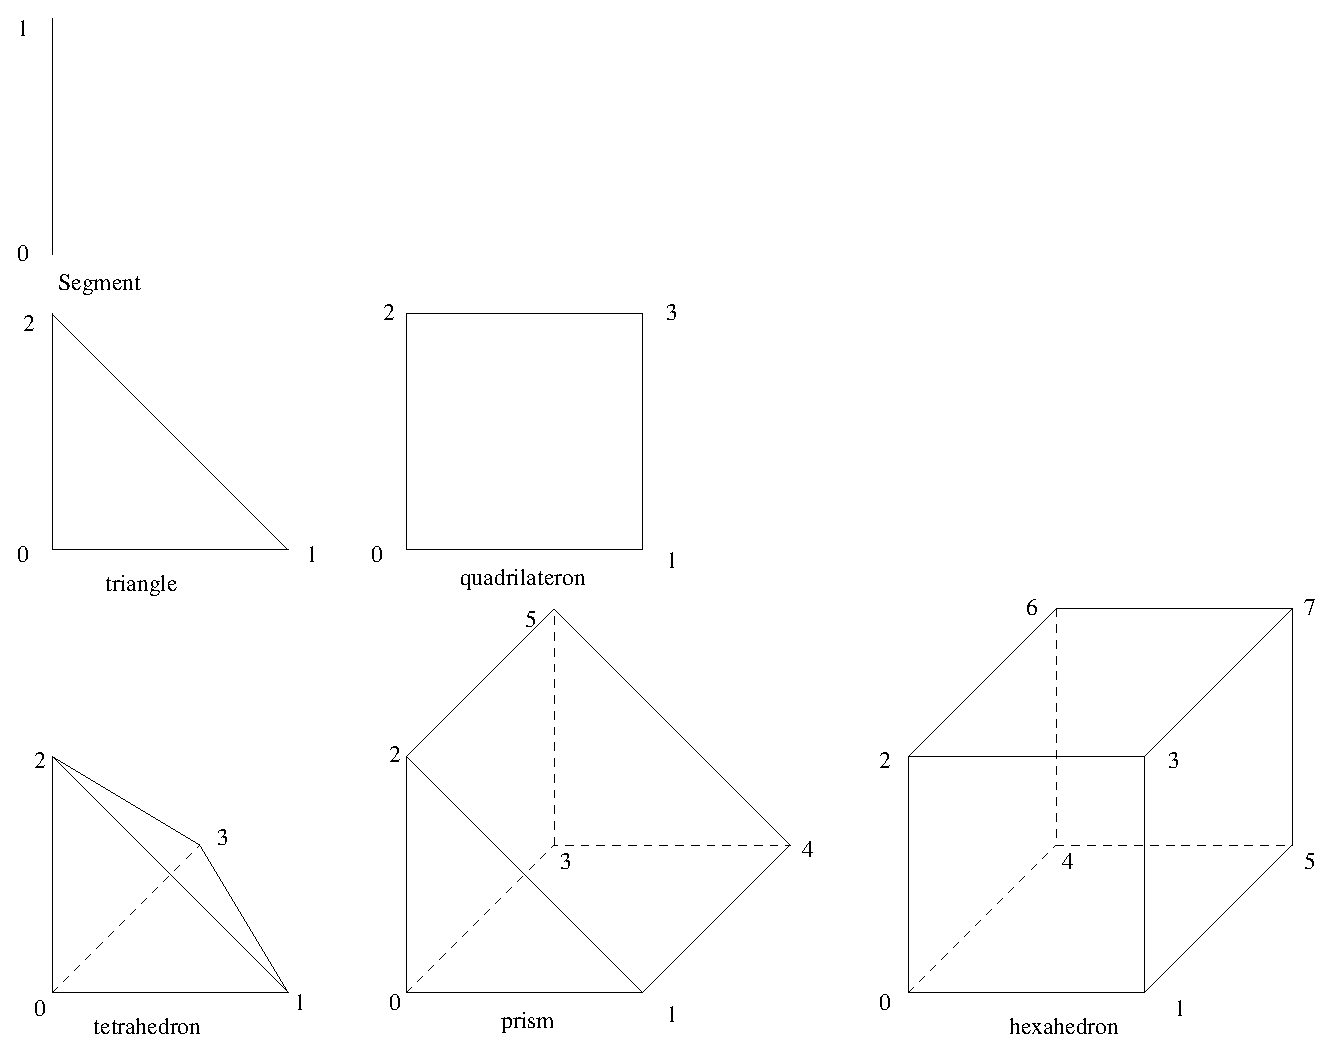
\includegraphics[width=15cm,angle=0]{getfemuserelem}}
    \htmlonly{\htmlimg{getfemuserelem.png}{vertex numeration for usual elements}}
  \end{center}
  \caption{ \it vertex numeration for usual elements }
  \label{fig:elem}
\end{figure}

\subsection{Remove an element from a mesh}
To remove an element from a mesh, simply use\\[0.5cm]
\index{GETFEM!mymesh.sup\_convex(i)}
\cpp{mymesh.sup\_convex(i); }\\[0.5cm]
where \cpp{i} is the index of the element.

\subsection{Simple structured meshes}

For parallelepiped domains, it is possible to obtain structured meshes with simplices, parallelepipeds or prisms elements from three functions defined in \cpp{getfem\_regular\_meshes.h}. \\[0.5cm]
\index{GETFEM!getfem::parallelepiped\_regular\_mesh}
\begin{cppcode}
  getfem::parallelepiped\_regular\_simplex\_mesh(mymesh, N, org, ivect, iref); \\
  getfem::parallelepiped\_regular\_prism\_mesh(mymesh, N, org, ivect, iref); \\
  getfem::parallelepiped\_regular\_mesh(mymesh, N, org, ivect, iref);
\end{cppcode}
where \cpp{mymesh} is a mesh variable in which the structured mesh will be built, \cpp{N} is the dimension (limited to 4 for simplices, 5 for prisms, unlimited for parallelepipeds), \cpp{org} is of type \cpp{bgeot::base\_node} and represents the origin of the mesh, \cpp{ivect} is an iterator on an array of \cpp{N} vectors to build the parallelepiped domain, \cpp{iref} is an iterator on an array of \cpp{N} integers representing the number of division on each direction. \\[0.5cm]
For instance, to build a mesh with tetrahedrons for a unit cube with $10�10�10$ cells one can write\\[0.5cm]
\begin{cppcode}
  getfem::mesh mymesh; \\
  bgeot::base\_node org(0.0, 0.0, 0.0); \\
  std::vector<bgeot::base\_small\_vector> vect(3); \\
  vect[0] = bgeot::base\_small\_vector(1.0, 0.0, 0.0); \\
  vect[1] = bgeot::base\_small\_vector(0.0, 1.0, 0.0); \\
  vect[2] = bgeot::base\_small\_vector(0.0, 0.0, 1.0); \\
  std::vector<int> ref(3); \\
  ref[0] = ref[1] = ref[2] = 10; \\
  getfem::parallelepiped\_regular\_simplex\_mesh(mymesh, 3, org, vect.begin(), ref.begin()); 
\end{cppcode}

Remark: \cpp{base\_node} and \cpp{base\_small\_vector} are almost identical, they are both ``small'' vector classes (they cannot store more than 16 elements), used to describe geometrical points, and geometrical vectors. Their memory footprint is lower than a \cpp{std::vector}.

\subsection{Mesh regions}
A mesh object can contain many \cpp{getfem::mesh\_region} objects. These objects are containers for a set of convexes and convex faces. They are used to define boundaries, or a partition of the mesh for parallel solvers, etc.
\begin{cppcode}
  mymesh.region(30).add(3);   // add convex 3 into region 30
  mymesh.region(30).add(4,3); // add face 3 of convex 4 into region 30
  mymesh.sup_convex(4);  // the correspounding entry will be removed from mesh.region(30)
  for (getfem::mr\_visitor i(mymesh.region(30)); !i.finished(); ++i) \{
    cout << "convex: " << i.cv() << " face:" << i.f() << endl;
  \}
\end{cppcode}

\subsection{Methods of the \cpp{getfem::mesh} object}

The list is not exhaustive.

\begin{ctableau}{|m{0.4\linewidth}|m{0.55\linewidth}|}{ll}\hline
  \cpp{mymesh.dim()} & main dimension of the mesh.  \\ \hline
  
  \cpp{mymesh.points\_index()} & gives a \cpp{dal::bit\_vector} object
  which represents all the indexes of valid points of a mesh (see in
  the following) \\ \hline
  
  \cpp{mymesh.points()[i]} & gives the point of index \cpp{i} (a
  \cpp{bgeot::base\_node} ). \\ \hline
  
  \cpp{mymesh.convex\_index()} & gives a \cpp{dal::bit\_vector} object
  which represents all the indexes of valid elements of a mesh (see in
  the following) \\ \hline
  
  \cpp{mymesh.structure\_of\_convex(i)} & gives the description of the
  structure of element of index \cpp{i}. The function return a
  \cpp{bgeot::pconvex\_structure}. \\ \hline
  
  \cpp{mymesh.structure\_of\_convex(i)\hspace{5em}->nb_faces()} & number
  of faces of element of index \cpp{i}. \\ \hline
  
  \cpp{mymesh.structure\_of\_convex(i)\hspace{5em}->nb\_points()} &
  number of vertices of element of index \cpp{i}. \\ \hline
  
  \cpp{mymesh.structure\_of\_convex(i)->dim()} & intrinsic dimension of
  element of index \cpp{i}. \\ \hline
  

  \cpp{mymesh.structure\_of\_convex(i)\hspace{5em}->nb\_points\_of\_face(f)}
  & number of vertices of the face of local index \cpp{f} of element
  of index \cpp{i}.\\ \hline
 

  \cpp{mymesh.structure\_of\_convex(i)\hspace{5em}->ind\_points\_of\_face(f)}
  & return a container with the local indexes of all vertices of the
  face of local index \cpp{f} of element of index \cpp{i}. For
  instance \cpp{mesh.structure\_of\_convex(i)
    ->ind\_points\_of\_face(f)[0]} is the local index of the first
  vertex. \\ \hline
  
  \cpp{mymesh.structure\_of\_convex(i)\hspace{5em}->face\_structure(f)}
  & gives the structure (a \cpp{bgeot::pconvex\_structure}) of local
  index \cpp{f} of element of index \cpp{i}.\\ \hline
  
  \cpp{mymesh.ind\_points\_of\_convex(i)} & gives a container with the
  global indexes of vertices of element of index \cpp{i}.\\ \hline
  
  \cpp{mymesh.points\_of\_convex(i)} & gives a container with the
  vertices of element of index \cpp{i}. This is an array of
  \cpp{bgeot::base\_node}.\\ \hline
  
  \cpp{mymesh.convex\_to\_point(ipt)} & gives a container with the
  indexes of all elements attached to the point of global index
  \cpp{ipt}.\\ \hline
  
  \cpp{mymesh.neighbours\_of\_convex(ic, f)} & gives a container with
  the indexes of all elements in \cpp{mesh} having the common face of
  local index \cpp{f} of element \cpp{ic} except element \cpp{ic}. \\ 
  \hline

  \cpp{mymesh.neighbour\_of\_convex(ic, f)} & gives the index of the
  first elements in \cpp{mesh} having the common face of
  local index \cpp{f} of element \cpp{ic} except element \cpp{ic}.
  return size_type(-1) if none is found. \\ 
  \hline

  \cpp{mymesh.is\_convex\_having\_neighbour(ic, f)} & return whether or not
  the element \cpp{ic} has a neighbour with respect to its face of
  local index \cpp{f}. \\ 
  \hline
  
  \cpp{mymesh.stat()} & print in \cpp{std::cout} main information on the
  mesh. \\ \hline
  
  \cpp{mymesh.clear()} & delete all elements and points from the mesh.
  \\ \hline

  \cpp{mymesh.optimize\_structure()} & compact the structure (renumbers points and convexes such that there is not hole in their numbering). \\ \hline
  
  \cpp{mymesh.trans\_of\_convex(i)} & geometric transformation of the
  element of index \cpp{i}. return a \cpp{bgeot::pgeometric\_trans}
  (see \cite{BASCOMP} for more details).  \\ \hline
  
  \cpp{mymesh.normal\_of\_face\_of\_convex(ic, f, pt)} & gives a
  \cpp{bgeot::base\_small\_vector} representing an outward normal to
  the element at the face of local index \cpp{f} at the point of local
  coordinates (coordinates in the element of reference) \cpp{pt}. The
  point \cpp{pt} has no influence if the geometric transformation is
  linear. This is not a unit normal, the norm of the resulting vector
  is the ratio between the surface of the face of the reference
  element and the the surface of the face of the real element. \\ 
  \hline
  
  \cpp{mymesh.convex\_quality\_estimate(ic)} & gives an rought estimate
  of the quality of element \cpp{ic}. \\ \hline
  
  \cpp{mymesh.convex\_radius\_estimate(ic)} & gives an estimate of the
  radius of element \cpp{ic}. \\ \hline 
  
  \cpp{mymesh.region(irg)} & return a \cpp{getfem::mesh\_region}. 
  The region is stored in the mesh, and can contain a set of convex
  numbers and or convex faces. \\ \hline

  \cpp{mymesh.has\_region(irg)} & returns true if the region of index \cpp{irg} has been created.\\ \hline
\end{ctableau}

The methods of the convexes/convex faces container \cpp{getfem::mesh\_region} are:
\begin{ctableau}{|m{0.4\linewidth}|m{0.55\linewidth}|}{ll}\hline
  \cpp{add(ic)} & add the convex of index \cpp{ic} to the region\\ \hline
  \cpp{add(ic,f)} & add the face number \cpp{f} of the convex \cpp{ic}\\ \hline
  \cpp{sup(ic)}, \cpp{sup(ic,f)} & remove the convex or the convex face from the region\\ \hline
  \cpp{is\_in(ic)}, \cpp{is\_in(ic,f)} & return true if the convex (or convex face) is in the region.\\ \hline
  \cpp{is\_only\_faces()} & return true if the region does not contain any convex.\\ \hline
  \cpp{is\_only\_convexes()} & return true if the region does not contain any convex face.\\ \hline
  \cpp{index()} & return a \cpp{dal::bit\_vector} containing the list of convexes which are stored (or whose faces are stored) in the region.\\ \hline
\end{ctableau}

Iteration over a \cpp{getfem::mesh\_region} should be done with \cpp{getfem::mr\_visitor}:
\begin{cppcode}
  getfem::mesh\_region &rg = mymesh.region(2);
  for (getfem::mr\_visitor i(rg); !i.finished(); ++i) \{
    cout << "contains convex " < < i.cv();
    if (i.is\_face()) cout  << "face " << i.f() << endl;
  \}
\end{cppcode}

\index{DAL!dal::bit\_vector} About the object \cpp{dal::bit\_vector},
which is very close to \cpp{std::bitset} but with additional
functionalities to represent a set of non negative integers. If
\cpp{nn} is declared to be a \cpp{dal::bit\_vector}, the two
instructions \cpp{nn.add(6)} or \cpp{nn[6] = true} are equivalent and
means that integer 6 is added to the set. In a same way
\cpp{nn.sup(6)} or \cpp{nn[6] = false} remove the integer 6 from the
set. The instruction \cpp{nn.add(6, 10)} adds the whole interval from
6 to 10 to the set (i.e. here 6, 7, 8, 9 and 10). To iterate on a
\cpp{dal::bit\_vector}, it is possible to use iterators as usual, but,
most of the time, as this object represents a set of integer, one just
wants to iterate on the integers included into the set. The simplest way to do that is to use the pseudo-iterator \cpp{dal::bv\_visitor}. 

For instance, here is the code to iterate on
the points of a mesh and print it to the standard output
\begin{cppcode}
  for (dal::bv\_visitor i(mymesh.points\_index()); !i.finished(); ++i)
    cout << "Point of index " << i << " of the mesh : " << mymesh.points()[i] << endl;
\end{cppcode}
The numeration of faces on usual elements is given in figure~\ref{fig:elemf}.
\begin{figure}[htb]
  \begin{center}
    \texonly{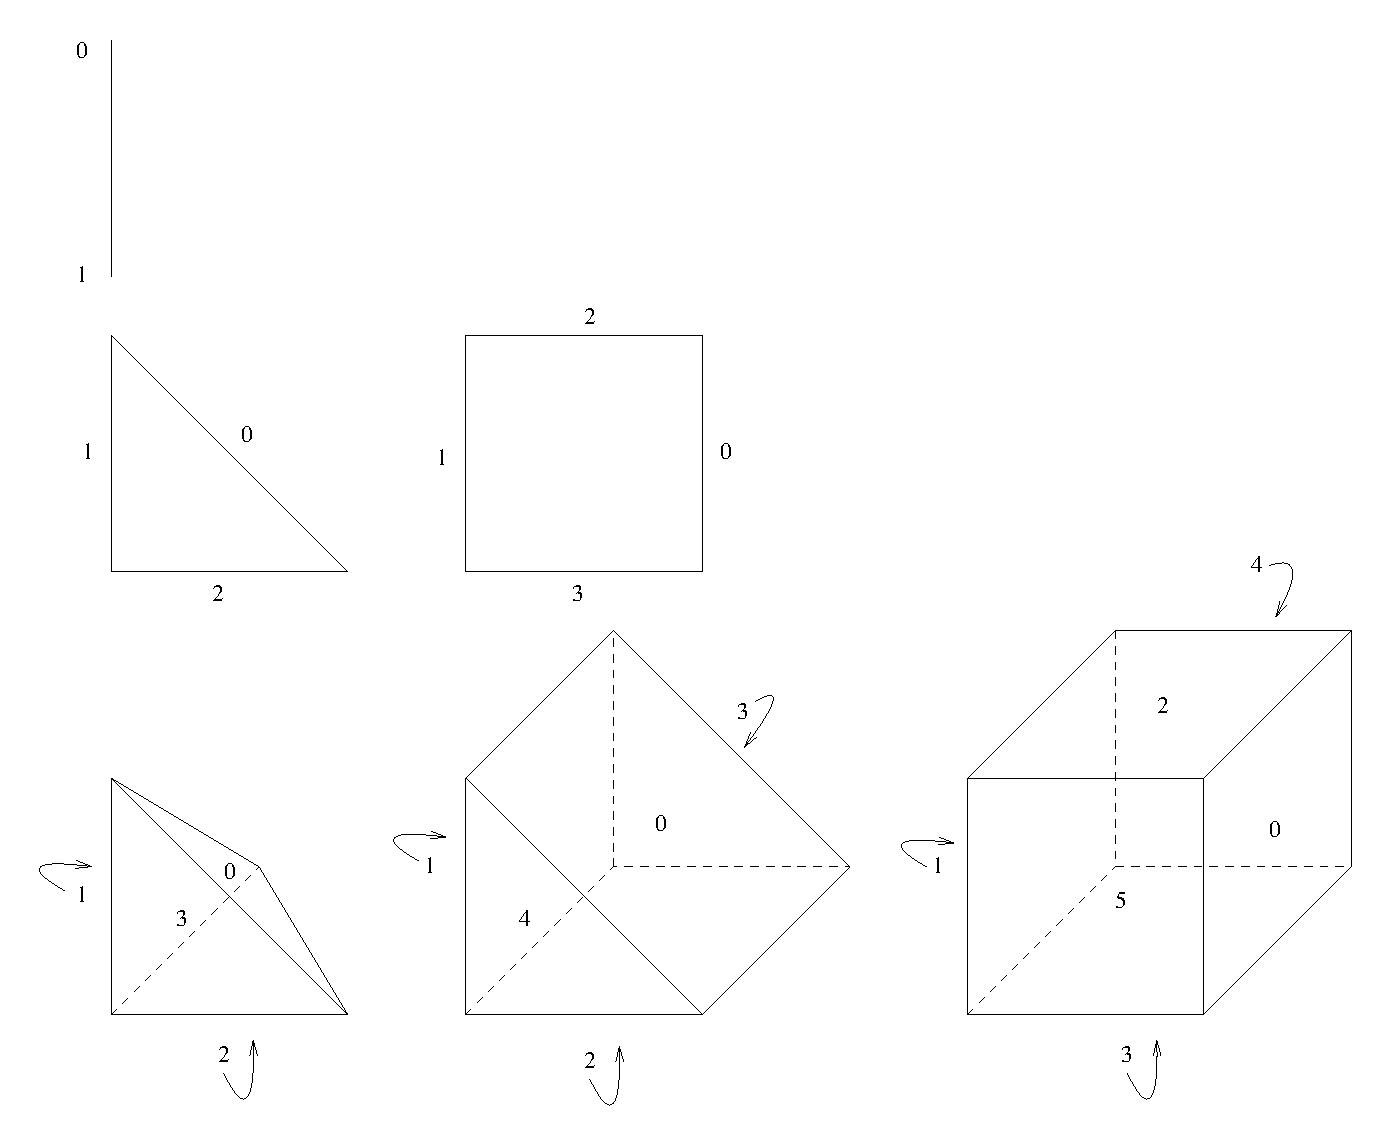
\includegraphics[width=15cm,angle=0]{getfemuserelemf}}
    \htmlonly{\htmlimg{getfemuserelemf.png}{faces numeration for usual elements}}
  \end{center}
  \caption{ \it faces numeration for usual elements }
  \label{fig:elemf}
\end{figure}

\subsection{Save, load and draw meshes}

(outadate section)

In \filename{getfem\_mesh.h}, two methods are defined to load meshes from file and write meshes to a file. \\[0.5cm]
\index{GETFEM!mymesh.write\_to\_file(name)}
\index{GETFEM!mymesh.read\_from\_file(name)}
\begin{ctableau}{|m{0.4\linewidth}|m{0.55\linewidth}|}{ll}\hline

  \cpp{mymesh.write\_to\_file(const std::string \&name)} & save the mesh into a file.\\ \hline

  \cpp{mymesh.read\_from\_file(const std::string \&name)} & load the mesh from a file.\\ \hline
\end{ctableau}

\subsection{example}

The following is an example of how to load a mesh and extract information on it.
\begin{cppcode}
  \#include <getfem\_mesh.h>
  
  getfem::mesh mymesh; 
  
  int main(int argc, char *argv[]) \{ 
    try \{ 
     
      // read the mesh from the file name given by the first argument 
      mymesh.read\_from\_file(std::string(argv[1])); 
     
      // List all the convexes
      dal::bit\_vector nn = mymesh.convex\_index(); 
      bgeot::size\_type i; 
      for (i << nn; i != bgeot::size\_type(-1); i << nn) \{
        cout << "Convex of index " << i << endl; 
        bgeot::pconvex\_structure cvs =  mymesh.structure\_of\_convex(i); 
        cout << "Number of vertices : " << cvs->nb\_points() << endl; 
        cout << "Number of faces : " << cvs->nb\_faces() << endl;
        for (bgeot::size\_type f = 0; f < cvs->nb\_faces(); ++f) \{
          cout << "face " << f << " has " << cvs->nb\_points\_of\_face(f); 
          cout << " vertices with local indexes : "; 
          for (bgeot::size\_type k = 0; k < cvs->nb\_points\_of\_face(f); ++k) 
          cout << cvs->ind\_points\_of\_face(f)[k] << " "; 
          cout << " and global indexes : ";
          for (bgeot::size\_type k = 0; k < cvs->nb\_points\_of\_face(f); ++k) 
            cout << mymesh.ind\_points\_of\_convex(i)[cvs->ind\_points\_of\_face(f)[k]] << " ";
        \}
     \}
     
   \} DAL\_STANDARD\_CATCH\_ERROR; // catches standard errors
 \}
\end{cppcode}

\section{Selecting finite element methods}
\index{GETFEM!getfem::mesh\_fem}
The description of a finite element method on a whole mesh is done thanks to the structure \cpp{getfem::mesh\_fem}, defined in the file \cpp{getfem\_mesh\_fem.h}. Basically, this structure describes the finite element method on each element of the mesh. It is possible to have an arbitrary number of finite element description for a single mesh. This is particularly necessary for mixed methods, but also to describe different data on the same mesh. One can instantiate a \cpp{getfem::mesh\_fem} object as follows\\[0.5cm]
\cpp{getfem::mesh\_fem mef(mymesh); }\\[0.5cm]
where \cpp{mymesh} is an already existing mesh. The structure will be linked to this mesh and will react when modifications will be done on it. \\[0.5cm]
It is possible to specify element by element the finite element method, so that element of mixed types can be treated, even if the dimensions are different. For usual elements, the connection between two elements is done when the two elements are compatibles (same degrees of freedom on the common face). A numeration of the degrees of freedom is automatically done with a Cuthill Mc Kee like algorithm. You have to keep in mind that there is absolutely no connection between the numeration of vertices of the mesh and the numeration of the degrees of freedom. Every \cpp{getfem::mesh\_fem} object has its own numeration. \\[0.5cm]
To select a particular finite element method on a given element, one can use \\[0.5cm]
\index{GETFEM!mef.set\_finite\_element(i, ppf)}
\cpp{mef.set\_finite\_element(i, ppf); }\\[0.5cm]
where \cpp{i} is the index of the element and \cpp{ppf} is the descriptor of the finite element method. Alternative forms of this member function are:
\begin{cppcode}
  void mesh\_fem::set\_finite\_element(const dal::bit\_vector &cvs, 
    getfem::pfem ppf);
  void mesh\_fem::set\_finite\_element(getfem::pfem pf);
\end{cppcode}
which set the finite elements for either the convexes listed in the \cpp{bit\_vector cvs}, or all the convexes of the mesh.

The list of all available descriptors of finite element methods is in the file \filename{getfem\_fem.h}. A short description is also given in \cite{BASCOMP}. 
Descriptors for finite element methods and integration methods are available thanks to the following function\\[0.5cm]
\index{GETFEM!getfem::fem\_descriptor("name")}\index{GETFEM!getfem::pfem}
\begin{cppcode}
  getfem::pfem ppf = getfem::fem\_descriptor("name of method");
\end{cppcode}
where \cpp{"name of method"} is to be chosen among the existing methods.
A name of a method can be retrieved thanks to the following functions\\[0.5cm]
\begin{cppcode}
  std::string femname = getfem::name\_of\_fem(ppf);
\end{cppcode}
A non exhautive list (see \cite{FEMLIST} for exhaustive lists) of finite element methods is given by
\begin{center} \begin{tabular}{|m{0.55\linewidth}|m{0.4\linewidth}|} \hline
{\tt getfem::ppolyfem getfem::PK\_fem(n, k)} & Classical $P_K$ methods on simplexes of dimension  {\tt n} with degree {\tt k} polynomials.\\ \hline
{\tt getfem::ppolyfem getfem::QK\_fem(n, k)} & Classical $Q_K$ methods on parallelepiped of dimension {\tt n}. Tensorial product of degree {\tt k} $P_K$ method on the segment. \\ \hline
{\tt getfem::ppolyfem getfem::PK\_prism\_fem(n, k)} & Classical methods on prism of dimension {\tt n}. Tensorial product of two degree {\tt k} $P_K$ method. \\ \hline
{\tt getfem::ppolyfem getfem::product\_fem( ppolyfem\;a, ppolyfem b)} & Tensorial product of the two polynomial finite element method {\tt a} and {\tt b}. \\ \hline
{\tt getfem::ppolyfem $\;$ getfem::P1\_nonconforming\_fem()} & Non conforming $P_1$ method on triangles. \\ \hline
\end{tabular} \end{center}


An alternative way to obtain a Lagrange polynomial fem suitable for a given geometric transformation is to use
\index{GETFEM!getfem::classical\_fem(pgt,degree)}\index{GETFEM!getfem::classical\_discontinuous\_fem(pgt,degree)}
\begin{cppcode}
 getfem::pfem getfem::classical\_fem(bgeot::pgeometric\_trans pg, short\_type degree);
 pfem getfem::classical\_discontinuous\_fem(bgeot::pgeometric\_trans pg, short\_type degree);
\end{cppcode}

The \cpp{mesh\_fem} can call directly these functions via:\index{GETFEM!getfem::set_classical\_finite\_element}\index{GETFEM!getfem::set\_classical\_discontinuous\_finite\_element}
\begin{cppcode}
  void mesh\_fem::set\_classical\_finite\_element(const dal::bit\_vector &cvs, 
    dim\_type fem\_degree);
  void mesh\_fem::set\_classical\_discontinuous\_finite\_element(const dal::bit\_vector &cvs, dim\_type fem\_degree);
  void mesh\_fem::set\_classical\_finite\_element(dim\_type fem\_degree);
  void mesh\_fem::set\_classical\_discontinuous\_finite\_element(dim\_type fem\_degree);                           
\end{cppcode}

\subsection{Examples}
For instance if one needs to have a description of a $P_1$ finite element method on a triangle, the way to set it is
\begin{cppcode}
 mef.set\_finite\_element(i, getfem::fem\_descriptor("FEM\_PK(2, 1)"));
\end{cppcode}
where \cpp{i} is still the index of the triangle. It is also possible to select a particular method directly on a set of element, passing to \cpp{mef.set\_finite\_element} a \cpp{dal::bit\_vector} instead of a single index. For instance
\begin{cppcode}
 mef.set\_finite\_element(mymesh.convex\_index(), getfem::fem\_descriptor("FEM\_PK(2, 1)"));
\end{cppcode}
selects the method on all the elements of the mesh.\\[0.5cm]
IMPORTANT: If the finite element represents an unknown for a vectorial
problem (such as the displacement for linear elasticity), one should
use \cpp{mef.set\_qdim(Q)} to set the target dimension (see
\cite{BASCOMP} for the definition of the target dimension $Q$).\\[0.5cm]
If the target dimension $Q$ is set to a value different of $1$, the
scalar FEMs (such as $P_k$ fems etc.) are automatically
``vectorized'', i.e. each scalar degree of freedom is duplicated $Q$
times, from the \cpp{mesh\_fem} object point of vue. To sum it up,
\begin{itemize}
\item if the fem of the $ith$ element is intrinsically a vector FEM,\\
 \cpp{mef.get\_qdim() == mef.fem\_of\_element(i)->target\_dim()} 
\\ and\\ \cpp{mef.nb\_dof\_of\_element(i) == mef.fem\_of\_element(i).nb\_dof()}.
\item if the fem has a \cpp{target\_dim} equal to $1$, \\
\cpp{mef.nb\_dof\_of\_element(i) == mef.get\_qdim()*mef.fem\_of\_element(i).nb\_dof()}.
\end{itemize}



\subsection{Other methods of the \cpp{mesh\_fem} object}

Once a finite element method is defined on a mesh, it is possible to obtain information on it with the following methods (the list is not exhaustive).\\[0.5cm]
\begin{center} \texonly{\begin{tabular}{|m{0.4\linewidth}|m{0.55\linewidth}|} \hline}\htmlonly{\xmlattributes*{table}{border}\begin{tabular}{l|l}}

  \cpp{mef.convex\_index()} & Set of indexes (a \cpp{dal::bit\_vector}) on which a finite element method is defined.  \\ \hline

  \cpp{mef.linked\_mesh()} & gives a reference to the linked mesh.  \\ \hline

  \cpp{mef.fem\_of\_element(i)} & gives a descriptor on the finite element method defined on element of index \cpp{i}.  \\ \hline

  \cpp{mef.nb\_dof\_of\_element(i)} & gives the number of degrees of freedom on the element of index \cpp{i}.  \\ \hline

  \cpp{mef.ind\_dof\_of\_element(i)} & gives a container (an array) with all the global indexes of the degrees of freedom of element of index \cpp{i}.  \\ \hline

  \cpp{mef.point\_of\_dof(i, j)} & gives a \cpp{bgeot::base\_node} which represents the point associated with the dof of local index \cpp{j} on element of index \cpp{i}.  \\ \hline

  \cpp{mef.point\_of\_dof(j)} & gives a \cpp{bgeot::base\_node} which represents the point associated with the dof of global index \cpp{j}.  \\ \hline

  \cpp{mef.reference\_point\_of\_dof(i, j)} & gives a \cpp{bgeot::base\_node} which represents the point associated with the dof of local index \cpp{j} on element of index \cpp{i} in the coordinates of the reference element.  \\ \hline

  \cpp{mef.first\_convex\_of\_dof(j)} & gives the index of the first element on which the degree of freedom of global index \cpp{j} is defined.  \\ \hline
  
  \cpp{mef.nb\_dof()} & gives the total number of different degrees of freedom.  \\ \hline

  \cpp{mef.get_qdim()} & gives the target dimension \cpp{Q}.  \\ \hline

  \cpp{mef.clear()} & Clear the structure, no finite element method is still defined.  \\ \hline

  \cpp{mef.dof_on_set(i)} & Return a \cpp{dal::bit_vector} which represent the indices of dof which are in the set of convexes or the set of faces of index \cpp{i} (see the \cpp{getfem::mesh} object).  \\ \hline

\end{tabular} \end{center}


\subsection{Obtaining generic mesh\_fems}

It is possible to use the function
\begin{cppcode}
  const mesh_fem &getfem::classical_mesh_fem(const getfem::mesh &mymesh, dim_type K);  
\end{cppcode}
to get a classical polynomial \cpp{mesh_fem} of order $K$ on the given \cpp{mymesh}.
The returned mesh_fem won't be destroyed until its linked_mesh is
destroyed. All the \cpp{mesh_fem} built by this function are stored
in a cache, which means that calling this function twice with
the same arguments will return the same \cpp{mesh_fem} object. A
consequence is that you should NEVER modify this mesh_fem!

\section{Selecting integration methods}
\index{GETFEM!getfem::mesh\_im}
The description of an integration method on a whole mesh is done thanks to the structure \cpp{getfem::mesh\_im}, defined in the file \cpp{getfem\_mesh\_im.h}. Basically, this structure describes the integration method on each element of the mesh. One can instantiate a \cpp{getfem::mesh\_im} object as follows\\[0.5cm]
\cpp{getfem::mesh\_im mim(mymesh); }\\[0.5cm]
where \cpp{mymesh} is an already existing mesh. The structure will be linked to this mesh and will react when modifications will be done on it. \\[0.5cm]
It is possible to specify element by element the integration method, so that element of mixed types can be treated, even if the dimensions are different. \\[0.5cm]
To select a particular integration method on a given element, one can use \\[0.5cm]
\index{GETFEM!mim.set\_integration\_method(i, ppi)}
\cpp{mef.set\_integration\_method(i, ppi); }\\[0.5cm]
where \cpp{i} is the index of the element and \cpp{ppi} is the descriptor of the integration method. Alternative forms of this member function are:
\begin{cppcode}
  void mesh\_fem::set\_integration\_method(const dal::bit\_vector &cvs, 
    getfem::pintegration\_method ppi);
  void mesh\_fem::set\_integration\_method(getfem::pintegration\_method ppi);
\end{cppcode}
which set the integration method for either the convexes listed in the \cpp{bit\_vector} cvs, or all the convexes of the mesh.

The list of all available descriptors of integration methods is in the file \filename{getfem\_integration.h}. \\[0.5cm]
Descriptors for integration methods are available thanks to the follofing function\\[0.5cm]
\index{GETFEM!getfem::int\_method\_descriptor("name")}\index{GETFEM!getfem::pintegration_method}
\begin{cppcode}
  getfem::pintegration_method ppi = getfem::int\_method\_descriptor("name of method");
\end{cppcode}
where \cpp{"name of method"} is to be chosen among the existing methods.
A name of a method can be retrieved thanks to the following function\\[0.5cm]
\begin{cppcode}
  std::string im\_name = getfem::name\_of\_int\_method(ppi);
\end{cppcode}
A non exhautive list (see \cite{FEMLIST} for exhaustive lists) of integration methods is given by:\\

Examples of exact integration methods:
\begin{center} \begin{tabular}{|m{0.55\linewidth}|m{0.4\linewidth}|} \hline
{\tt "IM\_EXACT\_SIMPLEX(n)"} & Description of the exact integration of polynomials on the simplex of reference of dimension {\tt n}. \\ \hline
\end{tabular}  
\begin{tabular}{|m{0.55\linewidth}|m{0.4\linewidth}|} \hline
{\tt "IM\_PRODUCT(a, b)"} & Description of the exact integration on the convex which is the direct product of the convex in {\tt a} and in {\tt b}.\\ \hline
\end{tabular}  
\begin{tabular}{|m{0.55\linewidth}|m{0.4\linewidth}|} \hline
{\tt "IM\_EXACT\_PARALLELEPIPED(n)"} & Description of the exact integration of polynomials on the parallelepiped of reference of dimension {\tt n}\\ \hline
\end{tabular}  
\begin{tabular}{|m{0.55\linewidth}|m{0.4\linewidth}|} \hline
{\tt "IM\_EXACT\_PRISM(n)"} & Description of the exact integration of polynomials on the prism of reference of dimension {\tt n}\\ \hline
\end{tabular} \end{center}

Examples of approximated integration methods:
\begin{center} \begin{tabular}{|m{0.55\linewidth}|m{0.4\linewidth}|} \hline
{\tt "IM\_GAUSS1D(k)" } & Description of the Gauss integration on a segment of order {\tt k}. \\ \hline
\end{tabular}  
\begin{tabular}{|m{0.55\linewidth}|m{0.4\linewidth}|} \hline
{\tt "IM\_NC(n,k)"} & Description of the integration on a simplex of reference of dimension {\tt n} for polynomials of degree {\tt k} with the Newton Cotes method (based on Lagrange interpolation).\\ \hline
\end{tabular}  
\begin{tabular}{|m{0.55\linewidth}|m{0.4\linewidth}|} \hline
{\tt "IM\_PRODUCT(a,b)"} & Build a method doing the direct product of methods {\tt a} and {\tt b}. \\ \hline
\end{tabular}  
\begin{tabular}{|m{0.55\linewidth}|m{0.4\linewidth}|} \hline
{\tt "IM\_TRIANGLE(2)"} & Integration on a triangle of order 2 with 3 points. \\ \hline
\end{tabular}
\begin{tabular}{|m{0.55\linewidth}|m{0.4\linewidth}|} \hline
{\tt "IM\_TRIANGLE(7)"} & Integration on a triangle of order 7 with 13 points. \\ \hline
\end{tabular} 
\begin{tabular}{|m{0.55\linewidth}|m{0.4\linewidth}|} \hline
{\tt "IM\_QUAD(2)"} & Integration on quadrilaterals of order 2 with 3 points. \\ \hline
\end{tabular}
\begin{tabular}{|m{0.55\linewidth}|m{0.4\linewidth}|} \hline
{\tt "IM\_TETRAHEDRON(5)"} & Integration on a tetrahedron of order 5 with 15 points. \\ \hline
\end{tabular} \end{center}

~\\

Remark: note that \texttt{IM\_QUAD(3)} is not able to integrate
exactly the base functions of the \texttt{FEM_QK(2,3)} finite element!
Since its base function are tensorial product of 1D polynomials of
degree 3, one would need to use \texttt{IM\_QUAD(7)} (6 is not
available). Hence \texttt{IM\_GAUSS\_PARALLELEPIPED(2,k)} should
always be prefered over \texttt{IM\_QUAD(2*k)} since it has less
integration points.

An alternative way to obtain integration methods: \index{GETFEM!getfem::classical\_exact\_im(pgt)}\index{GETFEM!getfem::classical\_approx\_im(pgt,degree)}
\begin{cppcode}
  getfem::pintegration\_method getfem::classical\_exact\_im(bgeot::pgeometric\_trans pgt);
  getfem::pintegration\_method getfem::classical\_approx\_im(bgeot::pgeometric\_trans pgt, dim\_type d);
\end{cppcode}
These functions return an exact (i.e. analytical) integration method, or select an approximate integration method which is able to integrate exactly polynamials of degree <= \cpp{d} (at least) for convexes defined with the specified geometric transformation.

\subsection{Methods of the \cpp{mesh\_im} object}

Once an integration method is defined on a mesh, it is possible to obtain information on it with the following methods (the list is not exhaustive).\\[0.5cm]
\begin{center} \texonly{\begin{tabular}{|m{0.4\linewidth}|m{0.55\linewidth}|} \hline}\htmlonly{\xmlattributes*{table}{border}\begin{tabular}{l|l}}

  \cpp{mim.convex\_index()} & Set of indexes (a \cpp{dal::bit\_vector}) on which an integration method is defined.  \\ \hline

  \cpp{mim.linked\_mesh()} & gives a reference to the linked mesh.  \\ \hline

  \cpp{mim.int\_method\_of\_element(i)} & gives a descriptor on the integration method defined on element of index \cpp{i}.  \\ \hline

  \cpp{mim.clear()} & Clear the structure, no finite element method is still defined.  \\ \hline

\end{tabular} \end{center}



\section{Linear algebra procedures} \label{sec:linalgproc}
The linear algebra library used by \gf is Gmm++ which is now a separate library. Please see the \WEB{http://www-gmm.insa-toulouse.fr/getfem/gmm_intro}{GMM++ user documentation}.\\

Note that Getfem++ includes (since release 1.7) its own version of SuperLU 3.0 ( \texttt{http://crd.lbl.gov/\tilda xiaoye/SuperLU/} ), hence a direct sparse solver is available out of the box.\\


A small interface to MUMPS ( \WEB{http://graal.ens-lyon.fr/MUMPS/}{http://graal.ens-lyon.fr/MUMPS/} or \WEB{http://www.enseeiht.fr/apo/MUMPS}{http://www.enseeiht.fr/apo/MUMPS} ) is also provided. See the file \cpp{gmm\_MUMPS\_interface.h}. In order to use MUMPS, you have to indicates some options to the configure shell:
\begin{cppcode}
  MUMPS_CFLAGS=" -I /path/to/MUMPS/include "
  MUMPS_LIBS=" F90 libraries and libs of MUMPS to be linked "
\end{cppcode}

For instance if you want to use the sequential version of MUMPS with double and complex double:
\begin{cppcode}
  MUMPS_CFLAGS=" -I /path/to/MUMPS/include "
  MUMPS_LIBS=" ...F90libs...  -L /path/to/MUMPS/lib -ldmumps -lzmumps -lpord -L /path/to/MUMPS/libseq -lmpiseq "
\end{cppcode}
where \textit{...F90libs...} are the libraries of the fortran compiler used to compile MUMPS (these are highly dependant on the fortran 90 compiler used, the ./configure script should detect the options relative to the default f90 compiler on your machine and display it -- for example, with the intel \texttt{ifort} compiler, it is ``\cpp{-L/opt/icc8.0/lib -lifport -lifcoremt -limf -lm -lcxa -lunwind -lpthread}'')

\section{Standard assembly procedures}

Procedures defined in the file \filename{getfem\_assembling.h} allow to assemble stiffness matrices, mass matrices and boundary conditions for a few amount of classical partial differential equation problems. All the procedures have vectors and matrices template parameters in order to be used with any matrix library.

\subsection{Laplacian (Poisson) problem}
\index{laplacian}
\index{Poisson problem}

An assembling procedure is defined to solve the problem
\texonly{\begin{eqnarray*}
  \Div (a(x)\ \Grad u(x)) = f(x), \ \ \text{in $\Omega$}, \\
  u(x) = U(x),  \ \ \text{on $\Gamma_{D}$}, \\
  \Frac{\partial u}{\partial \bf n} = F(x),  \ \ \text{ on $\Gamma_{N}$}, 
\end{eqnarray*}
}\htmlonly{
  \begin{equation*}
    \Div (a(x)\ \Grad u(x)) = f(x), \ \ \text{in $\Omega$},
  \end{equation*}
}
where $\Omega$ is an open domain of arbitrary dimension, $\Gamma_{D}$ and $\Gamma_{N}$ are parts of the boundary of $\Omega$, $u(x)$ is the unknown, $a(x)$ is a given coefficient, $f(x)$ is a given source term, $U(x)$ the prescribed value of $u(x)$ on $\Gamma_{D}$ and $F(x)$ is the prescribed normal derivative of $u(x)$ on $\Gamma_{N}$.
The function to be called to assemble the stiffness matrix is\\[0.5cm]
\index{GETFEM!getfem::asm\_stiffness\_matrix\_for\_laplacian}
\cpp{getfem::asm\_stiffness\_matrix\_for\_laplacian(SM, mim, mef1, mef2, A);} \\[0.5cm]
where \cpp{SM} is a matrix of any type having the right dimension (i.e. \cpp{me1.nb\_dof()}), \cpp{mim} is a variable of type  \cpp{getfem::mesh\_im} defining the integration method used, \cpp{mef1} is a variable of type \cpp{getfem::mesh\_fem} and should define the finite element method for the solution, \cpp{mef2}  is a variable of type \cpp{getfem::mesh\_fem} (possibly equal to \cpp{mef1}) describing the finite element method on which the coefficient $a(x)$ is defined, and \cpp{A} is the vector of the values of this coefficient on each degree of freedom of \cpp{mef2}. Both should use the same mesh. It is important to pay attention to the fact that the integration methods used to compute the elementary matrices are the ones declared in \cpp{mef1}. This integration method have to be chosen of sufficient order. The order has to be determined considering the degrees of element in \cpp{mef1}, in \cpp{mef2} and the geometric transformations for non-linear cases. Integration methods defined in \cpp{mef2} are ignored, hence you can use the dummy integration method \index{IM_NONE}{\tt IM\_NONE} with mef2.\\[0.5cm]
To assemble the source term, the  function to be called is\\[0.5cm]
\index{GETFEM!getfem::asm\_source\_term}
\cpp{getfem::asm\_source\_term(B, mim, mef1, mef2, V);} \\[0.5cm]
where \cpp{B} is a vector of any type having the right dimension (still \cpp{me1.nb\_dof()}), \cpp{mim} is a variable of type  \cpp{getfem::mesh\_im} defining the integration method used, \cpp{mef2}  is a variable of type \cpp{getfem::mesh\_fem} (possibly equal to \cpp{mef1}) describing the finite element method on which $f(x)$ is defined, \cpp{V} is the vector of the values of $f(x)$ on each degree of freedom of \cpp{mef2}.\\[0.5cm]
For the Neumann condition on $\Gamma_{N}$, the same function\\[0.5cm]
\cpp{getfem::asm\_source\_term(B, mim, mef1, mef2, V, nbound);} \\[0.5cm]
is used again, but an additional argument has been added: \cpp{nbound} is the index of the boundary in \cpp{mef1} (see previous section on how to describe a boundary) where the Neumann condition is applied. Hence the assembly is done on the indicated boundary, and no more on the whole domain. \cpp{mef2}  is a variable of type \cpp{getfem::mesh\_fem} describing the finite element method on which $F(x)$ is defined, \cpp{V} is the vector of the values of $F(x)$ on each degree of freedom of \cpp{mef2}.\\[0.5cm]
there is (at least) two manner to take into account the Dirichlet condition on $\Gamma_{D}$, changing the linear system or explicitly reduce to the kernel of the Dirichlet condition. For the first manner, the following function is defined \\[0.5cm]
\index{GETFEM!getfem::assembling\_Dirichlet\_condition}
\cpp{getfem::assembling\_Dirichlet\_condition(SM, B, mef1, nbound, V, N);} \\[0.5cm]
where \cpp{nbound} is the index of the boundary in \cpp{mef1} where the Dirichlet condition is applied, \cpp{V} is the vector of the values of $U(x)$ on each degree of freedom of \cpp{mef1} and \cpp{N} is the dimension for vectorial problems (should be \cpp{1} for scalar problems). This operation should be the last one because it transform the stiffness matrix \cpp{SM}. It works only for Lagrange elements. At the end, one obtains the discrete system
\begin{equation*} [SM] U = B, \end{equation*}
where $U$ is the discrete unknown.\\[0.5cm]

\T \newcommand{\tildeH}{\tilde{H}}
\W \newcommand{\tildeH}{HH}
\T \newcommand{\tildeR}{\tilde{R}}
\W \newcommand{\tildeR}{RR}
\T \newcommand{\tildeN}{\tilde{N}}
\W \newcommand{\tildeN}{NN}


For the second manner, one should use\\[0.5cm]
\index{GETFEM!getfem::asm\_dirichlet\_constraints}
\cpp{getfem::asm\_dirichlet\_constraints($\tildeH$, $\tildeR$, mim, mf\_u, mf\_mult, mf\_rh, $R$, nbound)}.\\[0.5cm]
See the Dirichlet condition as a general linear constraint that must
satisfy the solution $u$. This function does the assembly of 
Dirichlet conditions of type $\int_{\Gamma} u(x)v(x) = \int_{\Gamma}r(x)v(x)$ for all $v$ in the space of multiplier defined by \cpp{mf\_mult}. The fem \cpp{mf\_mult} could be often chosen equal to \cpp{mf\_u} except when \cpp{mf\_u} is too complex.
 
This function just assemble these
constraints into a new linear system $\tildeH u=\tildeR$, doing some
additional simplification in order to obtain a ``simple'' constraints
matrix.\\[0.5cm]

\index{GETFEM!getfem::Dirichlet\_nullspace} Then, one should
call \\[0.5cm]\cpp{ncols = getfem::Dirichlet\_nullspace($\tildeH$, $\tildeN$,
  $\tildeR$, Ud)},\\[0.5cm] which will return a vector $U_d$ which
satisfies the Dirichlet condition, and an orthogonal basis $\tildeN$ of the kernel of$\tildeH$. Hence, the discrete system that must be solved is
\begin{equation*} (\tildeN'[SM]\tildeN) U_{int}=\tildeN'(B-[SM]U_d),\end{equation*}
and the solution is $U=\tildeN U_{int}+U_d$.
The output matrix $\tildeN$ should be a $nbdof � nbdof$ (sparse) matrix but should be resized to \cpp{ncols} columns. The output vector $U_d$ should be a $nbdof$ vector.
A big advantage of this approach is to be generic, and do not prescribed for the finite element method \cpp{mf\_u} to be of Lagrange type. If \cpp{mf\_u} and 
\cpp{mf\_d} are different, there is implicitly a projection (with respect to the $L^2$ norm) of the data on the finite element \cpp{mf\_u}.

If you want to treat the more general scalar elliptic equation $\Div A(x)\nabla u$, where $A(x)$ is square matrix, you should use
\cpp{getfem::asm_stiffness_matrix_for_scalar_elliptic(M, mf,mfdata, A)}. The matrix data \cpp{A} should be defined on \cpp{mfdata}. It is expected as a vector representing a $n� n� nbdof$ tensor (in Fortran order), where $n$ is the mesh dimension of \cpp{mf}, and $nbdof$ is the number of dof of \cpp{mfdata}.

\subsection{Linear Elasticity problem}

the following function assembles the stiffness matrix for linear elasticity\\[0.5cm]
\index{GETFEM!getfem::asm\_stiffness\_matrix\_for\_linear\_elasticity}
\cpp{getfem::asm\_stiffness\_matrix\_for\_linear\_elasticity(SM, mim, mef1, mef2, LAMBDA, MU); } \\[0.5cm]
where \cpp{SM} is a matrix of any type having the right dimension (i.e. here \cpp{me1.nb\_dof()}), \cpp{mim} is a variable of type  \cpp{getfem::mesh\_im} defining the integration method used, \cpp{mef1} is a variable of type \cpp{getfem::mesh\_fem} and should define the finite element method for the solution, \cpp{mef2}  is a variable of type \cpp{getfem::mesh\_fem} (possibly equal to \cpp{mef1}) describing the finite element method on which the Lam{�} coefficient are defined, \cpp{LAMBDA} and \cpp{MU} are vectors of the values of Lam{�} coefficients on each degree of freedom of \cpp{mef2}. It is important to pay attention to the fact that the integration methods used to compute the elementary matrices is the ones declared in \cpp{mef1} and must be of sufficient order.\\[0.5cm]

CAUTION : Linear elasticity problem is a vectorial problem, so the target dimension of \cpp{mef1} (see \cpp{mef.set_qdim(Q)}) should be the same as the dimension of the mesh.\\[0.5cm]

In order to assemble source term, Neumann and Dirichlet conditions, same functions as in previous section can be used.

\subsection{Stokes Problem with mixed finite element method}

to be described ... (see the file \filename{getfem\_assembling.h} and the MATLAB interface).
 
\subsection{Assembling a mass matrix}

The following function allows to assemble a mass matrix for a finite element method\\[0.5cm]
\cpp{getfem::asm_mass\_matrix(M, mim, mef); } \\[0.5cm]
where \cpp{M} is a matrix of any type having the right dimension (i.e. here \cpp{me1.nb\_dof()}), \cpp{mim} is a variable of type  \cpp{getfem::mesh\_im} defining the integration method used, \cpp{mef} is a variable of type \cpp{getfem::mesh\_fem} and should define the finite element method. \cpp{mef} could represent a vectorial finite element method (i.e. \cpp{mef.get_qdim } $> 1$).
It is also possible to obtain  mass matrix on a boundary with the same function:
\cpp{getfem::asm_mass\_matrix(M, mim, mef, nbound); } \\[0.5cm]
where \cpp{nbound} is the index of the boundary in \cpp{mef}.


\section{Mesh refinement}

Mesh refinement with the Bank method (+ref) is available in dimension
1, 2 or 3 for simplex meshes (segments, triangles and tetrahedrons).
For a given object \cpp{mymesh} of type \cpp{getfem::mesh}, the method
\begin{cppcode}
  mymesh.Bank_refine(bv);
\end{cppcode}
refines the elements whose indices are stored in \cpp{bv} (a
\cpp{dal::bit\_vector} object). The conformity of the mesh is kept
thanks to additional refinement (the so called green triangles). Information about green triangles is stored on the mesh object to gather them for further refinements. (see Bank ...).


\begin{figure}[htb]
  \begin{center}
    \texonly{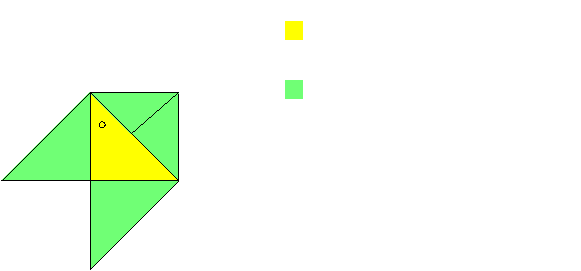
\includegraphics[width=10cm,angle=0]{getfemuserrefine.pdf}}
    \htmlonly{\htmlimg{getfemuserrefine.png}{Example of refinement}}
  \end{center}
  \caption{ \it Exemple of Bank refinement in 2D.}
  \label{fig:refine}
\end{figure}


Mesh refinement is most of the time coupled with an {\it a posteriori} error estimate. A basic error estimate is available in the file \cpp{getfem\_error\_estimate.h}. 
\begin{cppcode}
  error_estimate(mim, mf, U, err, cvlist);
\end{cppcode}
where \cpp{mim} is the integration method (a \cpp{getfem::mesh\_im} object),  \cpp{mf} is the finite element method on which the unknow has been computed (a \cpp{getfem::mesh\_fem} object), \cpp{U} is the vector of degrees of freedom of the unknow, \cpp{err} is a sufficiently large vector in which the error estimate is computed for each element of the mesh, and \cpp{cvlst} if a list of indices of element on which the error estimate should be computed (a \cpp{dal::bit\_vector} object).

This basic error estimate is only valid for order two problems and just compute the sum of the jump in normal derivative across the elements on each edge (for two-dimensional problems) or each face (for three-dimensional problems). This means that for each face $e$ of the mesh the following quantity is computed:

\texonly{$$}
\htmlonly{$}
\int_e |\hspace{0.01em}[\hspace{-0.12em}[ \partial_n u ]\hspace{-0.12em}]\hspace{0.01em}|^2 d \Gamma,
\htmlonly{$}
\texonly{$$}

where $[\hspace{-0.12em}[ \partial_n u ]\hspace{-0.12em}]$ is the jump of the normal derivative.
Then, for each element the mean value is computed with respect to its faces and stored in the vector \cpp{err}. This basic error estimate can be taken as a model for more elaborated ones.



\section{Compute arbitrary elementary matrices - generic assembly procedures}
As it can be seen in the file \filename{getfem_assembling.h}, all the
previous assembly procedures use a \cpp{generic_assembly} object and
provide it an adequate description of what must be done. For example, 
the assembly of a volumic source term for a scalar FEM is done with the following excerpt of code:
\index{GETFEM!getfem::generic_assembly}
\begin{cppcode}
  getfem::generic_assembly assem;
  assem.push_im(mim);
  assem.push_mf(mf);
  assem.push_mf(mfdata);
  assem.push_data(F);
  assem.push_vec(B);
  assem.set("Z=data(#2); V(#1)+=comp(Base(#1).Base(#2))(:,j).Z(j);");
  assem.assembly();
\end{cppcode}

The first instructions declare the object, and set the data that it
will use: a \cpp{mesh\_im} object which holds the integration methods,
two \cpp{mesh\_fem} objects, the input data \cpp{F}, and the
destination vector \cpp{B}.

The input data is the vector $F$, defined on \cpp{mfdata}. One wants
to evaluate $\sum_{j} f_j (\int_\Omega \phi^i \psi^j)$. The instruction must be seen as
something that will be executed for each convex \cpp{cv} of the mesh.
The terms \cpp{\#1} and \cpp{\#2} refer to the first \cpp{mesh\_fem} and
the second one (i.e. \cpp{mf} and \cpp{mfdata}).  The instruction
\cpp{Z=data(\#2);} means that for each convex, the ``tensor'' \cpp{Z}
will receive the values of the first data argument provided with
\cpp{push\_data}, at indexes corresponding to the degrees of freedom
attached to the convex of the second (\cpp{\#2}) \cpp{mesh_fem} (here,
\cpp{Z = F[mfdata.ind_dof_of_element(cv)]}.

The part \cpp{V(\#1)+=\ldots} means that the result of the next expression
will be accumulated into the output vector (provided with
\cpp{push\_vec}). Here again, \cpp{\#1} means that we will write the
result at indexes corresponding to the degrees of freedom of the
current convex with respect to the first (\cpp{\#1}) \cpp{mesh_fem}.

The left hand side \cpp{comp(Base(\#1).Base(\#2))(:,j).Z(j)} contains
two operations. The first one is a computation of a tensor on the
convex: \cpp{comp(Base(\#1).Base(\#2))} is evaluated as a 2-dimensions
tensor, $\int\phi^i \psi^j$, for all degrees of freedom $i$ of \cpp{mf} and $j$
of \cpp{mfdata} attached to the current convex. The next part is a
reduction operation, \cpp{C(:,j).Z(j)}: each named index (here $j$) is
summed, i.e. the result is $\sum_j c_{i,j} z_j$.

The integration method used inside \cpp{comp(Base(\#1).Base(\#2))} is
taken from \cpp{mim}. If you need to use integration methods from
another \cpp{mesh\_im} object, you can specify it as the first argument
of \cpp{comp}, for example \cpp{comp(\%2, Base(\#1).Grad(\#2))} will use
the second \cpp{mesh\_im} object (New in getfem++-2.0).

An other example is the assembly of the stiffness matrix for a vector Laplacian:
\begin{cppcode}
  getfem::generic_assembly assem;
  assem.push\_im(mim);
  assem.push_mf(mf);
  assem.push_mf(mfdata);
  assem.push_data(A);
  assem.push_mat(SM);
  assem.set("a=data$1(#2);"
            "M$1(\#1,\#1)+=sym(comp(vGrad(\#1).vGrad(\#1).Base(\#2))(:,j,k,:,j,k,p).a(p))");
  assem.assembly();
\end{cppcode}

Now the output is written in a sparse matrix, inserted with
\cpp{assem.push_mat(SM)}. The \cpp{\$1} in \cpp{M\$1(\#1,\#1)} just
indicates that we refer to the first matrix ``pushed'' (it is
optional, but if the assembly builds two matrices, the second one must
be referred this way). The \cpp{sym} function ensure that the result
is symmetric (if this is not done, some round-off errors may cancel
the symmetricity). Next, the \cpp{comp} part evaluates a 7D tensor,
\begin{equation*}\int\partial_k \varphi^{i}_{j} \partial_l \varphi^m_n \psi^p,\end{equation*} where
$\varphi^i_j$ is a $jth$ component of the $ith$ base function of \cpp{mf}
and $\psi^p$ is a (scalar) base function of the second \cpp{mesh_fem}.
Since we want to assemble
\begin{equation*}\int a(x).\nabla\phi^i.\nabla\phi^j,\quad\text{with}\quad a(x)=\sum_p a^p \psi^p(x),\end{equation*}
the reduction is:
\begin{equation*}\sum_{j,k,p}\left(\int \partial_k\varphi^{i}_{j} \partial_k\varphi^m_j \psi^p\right)a^p\end{equation*}
In the \cpp{comp} function, \cpp{vGrad} was used instead of \cpp{Grad} since we
said that we were assembling a {\em vector} Laplacian: that is why
each \cpp{vGrad} part has three dimensions (dof number, component
number, and derivative number). For a scalar Laplacian, we could have
used \cpp{comp(Grad(\#1).Grad(\#1).Base(\#2))(:,k,:,k,p).a(p)}. But the
vector form has the advantage to work in both vector and scalar case.

The last instruction, \cpp{assem.assembly()}, does evaluate the
expression on each convex. For an assembly over a boundary just call
\cpp{assem.assembly(rg)}, where \cpp{rg} is a
\cpp{getfem::mesh\_region} object.  \cpp{rg} might also be a number, in that
case the mesh region taken into account is
\cpp{mim.linked\_mesh().region(rg)}.


The third example shows how to compute the $L^2$ norm of a scalar or vector field on a mesh boundary:
\begin{cppcode}
    assem.push_im(mim);
    assem.push_mf(mf);
    assem.push_data(U);
    std::vector<scalar_type> v(1);
    assem.push_vec(v);
    assem.set("u=data(#1); V()+=u(i).u(j).comp(vBase(#1).vBase(#1))(i,k,j,k)");
    assem.assembly(boundary_number);
\end{cppcode}
This one is easy to read. When \cpp{assembly} returns, \cpp{v[0]} will contain 
\begin{equation*}\sum_{i,j,k}\left(\int_{boundary} u_i \varphi^{i}_{k} u_j \varphi^j_k \right)\end{equation*}


The fourth and last example shows an (sub-optimal) assembly of the linear elasticity problem with a complete Hooke tensor:
\begin{cppcode}
 assem.set("h=data\$1(qdim(\#1),qdim(\#1),qdim(\#1),qdim(\#1),\#2);"
           "t=comp(vGrad(\#1).vGrad(\#1).Base(\#2));"
           "e=(t\{:,2,3,:,5,6,:\}+t\{:,3,2,:,5,6,:\}+t\{:,2,3,:,6,5,:\}+t\{:,3,2,:,6,5,:\})/4;"
           "M(\#1,\#1)+= sym(e(:,j,k,:,m,n,p).h(j,k,m,n,p))");
\end{cppcode}
The original equations are:
\begin{equation*}\int\varepsilon(\varphi^i):\sigma(\phi^j),\quad\text{with}\quad
\sigma(u)_{ij}=\sum_{kl} h_{ijkl}(x) \varepsilon_{kl}(u)\end{equation*}
where $h$ is the Hooke tensor, and ':' means the scalar product between matrices.
Since we assume it is not constant, $h$ is given on the second \cpp{mesh_fem}: $h_{ijkl}(x)=\sum_p h_{ijkl}^p \psi^p$.  Hence the first line
declares that the first data ``pushed'' is indeed a five-dimensions
tensor, the first fourth ones being all equal to the target dimension
of the first \cpp{mesh_fem}, and the last one being equal to the
number of degrees of freedom of the second \cpp{mesh_fem}.  The \cpp{comp} part still computes the same 7D tensor than for the
vector Laplacian case.  From this tensor, one evaluates
$\varepsilon(\varphi^i)_{jk}\varepsilon(\phi^l)_{mn}\psi^p$ via permutations, and finally the
expression is reduced against the hook tensor.

{\bf availaible operations inside the \cpp{comp} command}

\begin{itemize}

\item[\cpp{Base(\#i)}] : evaluate the value of the base functions of
  the \textit{ith} \cpp{mesh\_fem}

  \item[\cpp{Grad(\#i)}] : evaluate the value of the gradient of the
    base functions of the \textit{ith} \cpp{mesh\_fem}

  \item[\cpp{Hess(\#i)}] : evaluate the value of the Hessian of the
    base functions of the \textit{ith} \cpp{mesh\_fem}

  \item[\cpp{Normal()}]: (New in getfem++-1.7) evaluate the unit
    normal (should not be used for volumic integrations !)

  \item[\cpp{NonLinear\$x(\#mf1,\ldots\#mfn)}] : (New in getfem++-1.7)
    evaluate the \textit{xth} non-linear term (inserted with
    \cpp{push\_nonlinear\_term(pnonlinear\_elem\_term)}) using the listed
    mesh\_fem objects.
  
  \item (New in getfem++-1.7) you may reference any data object inside
    the \cpp{comp} command, and perform reductions inside the
    \cpp{comp()}. This feature is mostly interesting for speeding up
    assembly of nonlinear terms (see getfem\_nonlinear\_elasticy.h for
    an example of use).

  \item[\cpp{GradGT()}, \cpp{GradGTInv}] : evaluate the gradient (and
    its inverse) of the geometric transformation of the current
    convex.

\end{itemize}

{\bf others operations}

Slices may be mixed with reduction operations \cpp{t(:,4,i,i)} takes a
slice at index 4 of the second dimension, and reduces the diagonal of
dimension 3 and 4. {\em Please note that index numbers for slices
  start at 1 and not 0 !!}

\cpp{mdim(\#2)} is evaluated as the mesh dimension associated to the
second \cpp{mesh_fem}, while \cpp{qdim(\#2)} is the target dimension of
the \cpp{mesh_fem}.

The diagonal of a tensor can be obtained with \cpp{t\{:,:,3,3\}} (which
is strictly equivalent to \cpp{t\{1,2,3,3\}}: the colon is just here to
improve the readability). This is the same operator than for
permutation operations. Note that \cpp{t\{:,:,1,1\}} or \cpp{t\{:,:,4,4\}}
are not valid operations.

The \cpp{print} command can be used to see the tensor: \cpp{"print
  comp(Base(\#1));"} will print the integrals of the base functions for
each convex.

If there is more than one data array, output array or output sparse
matrix, one can use \cpp{data\$2, data\$3, V\$2, M\$2,}\ldots

\section{Incorporate new finite element methods in \gf }

Basically, It is sufficient to describe an element on the reference
element, i.e. to describe each base function of each degree of
freedom. Vectorial elements elements are partially supported \ldots
(supported by the finite element kernel but none vector element is
implemented for now).

To be done ... please read \cite{BASCOMP} for more details and see the
file \filename{getfem\_fem.cc} for practical implementation.

\section{Incorporate new approximated integration methods in \gf }

A perl script automatically incorporates new cubature methods from a
description file. You can see in the directory {\tt cubature} such
description files (with extension {\tt.IM}) . For instance for {\tt
  IM_TETRAHEDRON(5)} the following file describes the method:

\begin{alltt}
NAME = IM_TETRAHEDRON(5)
N = 3
GEOTRANS = GT_PK(3,1)
NBPT = 4
0, 0.25, 0.25, 0.25, 0.008818342151675485
1, 0.31979362782962991, 0.31979362782962991, 0.31979362782962991, 0.011511367871045398 
1, 0.091971078052723033, 0.091971078052723033, 0.091971078052723033, 0.01198951396316977
1, 0.056350832689629156, 0.056350832689629156, 0.44364916731037084, 0.008818342151675485
NBF = 4
IM_TRIANGLE(5)
IM_TRIANGLE(5)
IM_TRIANGLE(5)
IM_TRIANGLE(5)
\end{alltt}


where {\tt NAME} is the name of the method in \gf (constant integer
parameter are allowed), {\tt N} is the dimension, {\tt GEOTRANS}
describes a valid geometric transformation of \gf. This geometric
transformation just defines the reference element on which the
integration method is described. {\tt NBPT} is the number of
integration node definitions. Integration node definitions include a
symmetry definition such that the total number of integration nodes
would be greater than {\tt NBPT}.


Composition of the integration node definition :
\begin{itemize}
  \item an integer : 0 = no symmetry, 1 = full symmetric (x6 for a triangle, x4 for a quadrangle, x24 for a tetrahedron ...),
  \item the {\tt N} coordinates of the integration node,
  \item the load.
\end{itemize}

{\tt NBF} is the number of faces of the reference element (should correspond to {\tt GEOTRANS}). Then follows an already existing integration method for each face (each on a line). This is necessary to make integrations on boundaries.


The file format is inspired from \cite{EncyclopCubature}.

\section{Support for Xfem methods}
\index{GETFEM!Xfem} Xfem are finite element method with a particular
enrichment with non-polynomials functions (see \cite{Xfem} for
instance). The file {\tt getfem_Xfem.h} gives a support for this kind
of method. Any ($\tau$-equivalent) valid finite element method can be
extended. If {\tt pf} is a valid descriptor of a finite element
method, one can build a Xfem with the declaration
\begin{cppcode}
  Xfem  xf(pf);
\end{cppcode}
then one adds a global function with
\begin{cppcode}
  xf.add_function(pXf, pXg, pXh, ind);
\end{cppcode}
where {\tt pXf} should be a pointer on a type derived from the object
{\tt virtual_Xfem_func} representing the global function, {\tt pXg}
should be a pointer on a type derived from the object {\tt
  virtual_Xfem_grad} representing the global function gradient, {\tt
  pXh} is an optional parameter (only for fourth order derivative
problems) which should be a pointer on a type derived from the object
{\tt virtual_Xfem_hess} representing the global function Hessian and
{\tt ind} is an index which should correspond to this function to
identify the degrees of freedom (this should be different for each
function added). It is possible to add an arbitrary number of global
functions. The total number of degrees of freedom of the Xfem is the
number of degrees of freedom of the initial fem times $N_f+1$ where
$N_f$ is the number of global functions added.


If $\varphi_i$ for $i=1..N_d$ are the basis functions of {\tt pf} and $f_j$
for $j=1..N_f$ the additional global functions, the basis functions of
the Xfem are the basis function $\varphi_i$ for $i=1..N_d$ and the basis
functions $f_j\varphi_i$ for $i=1..N_d$ and $j=1..N_f$. From an element to
another and for each function $f_j$, the corresponding degrees of
freedom are connected in a same manner as the corresponding degrees of
freedom of {\tt pf}.


Most of the time, one only needs an enrichment on a subset of node of
the original element. If it is so, one should a posteriori eliminate
the unwanted extra-dofs.

\section{Interpolation of a finite element method on non-matching meshes}


(evolution of \cpp{virtual\_link\_fem}) A special finite element method
is defined in \filename{getfem\_interpolated\_fem.h} which is not a real
finite element method but allows to interpolate a finite element
method defined on another mesh. When an assembling procedure has
different finite element methods as arguments, the mesh on which those
methods are defined should be the same. If you need to assemble a
matrix with finite element methods defined on different meshes, you
may use the finite element methods.


\index{GETFEM!getfem::interpolated\_fem}
\cpp{getfem::new_interpolated\_fem(getfem::mesh\_fem mf, getfem::mesh\_im mim) }\\[0.2cm]
Because each base function of the finite element method has to be
interpolated, such a computation can be a heavy procedure. By default,
the interpolated fem object store the interpolation.

The interpolation is made on each Gauss point of the integration
methods of \cpp{mim}, so that you have to use these integration
methods in the assembling procedures.

For instance if you need to compute the mass matrix between to
different finite element methods defined on two different meshes, this
is an example of code which interpolate the second f.e.m. on the mesh
of the first f.e.m., assuming that \cpp{mf} describes the finite
element method and \cpp{mim} is the chosen integration method.

\begin{cppcode}
  getfem::mesh\_fem mf\_interpole(mf.linked\_mesh());
  pfem ifem = getfem::new_interpolated\_fem(mf, mim);
  dal::bit\_vector nn = mf.convex\_index();
  mf\_interpole.set\_finite\_element(nn, ifem);
  getfem::asm\_mass\_matrix(SM1, mim, mf1, mf\_interpole);
  del_interpolated_fem(ifem);
\end{cppcode}

The object pointed by \cpp{ifem} contains all the information
concerning the interpolation. It could use a lot of memory. As pfem is
a smart pointer (a boost instrusive pointer, see
http://www.boost.org/), the interpolated fem will be automatically be
destroyed when the last pointer on it will be destroyed. To obtain a
better accuracy, it is better to refine the integration method (with
\cpp{IM_STRUCTURED_COMPOSITE} for instance) rather than improve its
order.

\subsection{mixed methods with different meshes}
  to be described ...
\subsection{mortar methods}
  to be described ...


\section{Compute $L^2$ and $H^1$ norms}

The file \filename{getfem\_assembling.h} defines the functions to compute $L^2$ and $H^1$ norms of a solution. The following functions compute the different norms\\[0.5cm]
\index{GETFEM!asm_L2\_norm(mef, U)}
\index{GETFEM!asm_H1\_norm(mef, U)}
\cpp{getfem::asm_L2\_norm(mef, U); } \\[0.5cm]
\cpp{getfem::asm_H1\_semi\_norm(mef, U); } \\[0.5cm]
\cpp{getfem::asm_H1\_norm(mef, U); } \\[0.5cm]
where \cpp{mef} is a variable of type \cpp{getfem::mesh\_fem} and describes the finite element method on which the solution is defined, \cpp{U} is the vector of values of the solution on each degree of freedom of \cpp{mef}. The size of  \cpp{U} should be \cpp{mef.nb\_dof()}.\\[0.5cm]

\section{Compute derivatives}

The file \filename{getfem\_derivatives.h}  defines the following function to compute the gradient of a solution\\[0.5cm]
\index{GETFEM!getfem::compute\_gradient}
\cpp{getfem::compute\_gradient(mim, mef1, mef2, U, V); }\\[0.5cm]
where \cpp{mef1} is a variable of type \cpp{getfem::mesh\_fem} and describes the finite element method on which the solution is defined, \cpp{mef2} describes the finite element method to compute the gradient, \cpp{U} is a vector representing the solution and should be of size \cpp{mef1.nb\_dof()}, \cpp{V} is the vector on which the gradient will be computed and should be of size
\cpp{N * mef2.nb\_dof()} where \cpp{N} is the dimension of the domain. IMPORTANT : This function only work when \cpp{mef2} is a Lagrange element. This element should be, most of the time, a discontinuous Lagrangian element, because for usual element (for instance \cpp{getfem::PK\_discontinuous\_fem(n, k)}), the gradient is not continuous.

\section{Export and view a solution}

If you have installed the Matlab interface, you can simply use \cpp{mesh_fem::write_to_file} and save the solution as a plain text file, and then, load them into Matlab. See the getfem-matlab interface documentation for more details.

Two other file formats are supported for export: the \WEB{http://http://www.kitware.com/}{VTK file format} and the \WEB{http://www.opendx.org/}{OpenDX} file format.

Examples of use can be found in the examples of the tests directory. 

\subsection{Mesh slices}
Getfem++ provides a \cpp{getfem::mesh_slice} class,
with support general slicing operations on a mesh (slicing with a
plane, half-space, cylinder, sphere, isosurfaces, union or
intersection of slices, etc..). A slice object may be considered as a
P1 discontinuous \cpp{mesh_fem} with fast interpolation ability.  See
\filename{getfem_mesh_slices.h} for more information, and the
\filename{gf_slice.cc} file of the getfem-matlab interface for an
example of use.

\section{Interpolation on different meshes}

The file \filename{getfem\_export.h} defines the following function to interpolate a solution from a mesh and a finite element method  to another mesh and another Lagrange finite element method.\\[0.5cm]
\index{GETFEM!getfem::interpolation\_solution}
\cpp{getfem::interpolation\_solution(mef1, mef2, U, V); }\\[0.5cm]
where \cpp{mef1}  is a variable of type \cpp{getfem::mesh\_fem} and describes the finite element method on which the solution is defined, \cpp{mef2} is the finite element method on which the solution will be interpolate,  \cpp{U} is a vector representing the solution and should be of size \cpp{mef1.nb\_dof()}, \cpp{V} is a vector on which the interpolation will be computed and should be of size \cpp{mef2.nb\_dof()}. IMPORTANT : \cpp{mef2} should be of Lagrange type for the interpolation to makes sense but the meshes linked to \cpp{mef1} and \cpp{mef2} may be different (and this is the interest of this function). There is no restriction for the dimension of the domain.\\

If you need to make more than one interpolation between the same finite element methods, it is better to use the function
\cpp{getfem::interpolation\_solution(mef1, mef2, M); }\\[0.5cm]
where \cpp{M} is a row matrix which will be filled with the linear map representing the interpolation (i.e. such that \cpp{V = MU}). The matrix should have the right dimensions (i.e. \cpp{mef2.nb\_dof()} x \cpp{mef1.nb\_dof()}).



\section{The model bricks}
\index{model bricks}
 Although it is possible to use assembly
procedures on their own to make your finite element programs, it is
now possible to use predefined bricks to build up very quickly a
certain number of models. Most of the bricks are defined in
\cpp{getfem_modeling.h}

A model brick is basically an object which modifies a global tangent
matrix and its associated right hand side. Typical modifications are
insertion of the stiffness matrix for the problem considered (linear
elasticity, laplacian, \ldots), handling of a set of contraints, Dirichlet
condition, addition of a source term to the right hand side etc. The
global tangent matrix and its right hand side are stored in a
\cpp{model\_state} structure.

\subsection{The model state variable}
\index{GETFEM!getfem::model\_state} The \cpp{model_state} object is an
object which stores the state of the system and the tangent system
with eventual constraints. There are two predefined \cpp{model_state} types:
\begin{cppcode}
  getfem::standard_model_state
  getfem::standard_complex_model_state
\end{cppcode}
The second one is for models with complex degrees of freedom like
Helmholtz problem. These two predefined \cpp{model_state} type are built
with the following predefined sparse matrices and plain vectors:
\begin{cppcode}
  getfem::modeling_standard_sparse_matrix (gmm::col_matrix<gmm::rsvector<double> >)
  getfem::modeling_standard_plain_vector (std::vector<double>)
  getfem::modeling_standard_complex_sparse_matrix (gmm::col_matrix<gmm::rsvector<std::complex<double> > >)
  getfem::modeling_standard_complex_plain_vector (std::vector<std::complex<double> >)
\end{cppcode}
But you can define your own model state type with arbitrary types of sparse matrices and plain vectors (see the file {\tt getfem_modeling.h})

\subsection{Basic properties of a brick}

A brick represents a basic problem (elasticity, Helmholtz, Poisson
problems ...) or a modifier of such problems (addition of a Dirichlet
or Neumann condition, source term, incompressibility term ...).  Each
brick will participate on the global linear system to be solved (the
tangent system for non linear problem).
A brick is an object which derives from \cpp{mdbrick_abstract<MODEL_STATE>} with 
the following virtual methods to be defined:\\[0.5cm]

\begin{ctableau}{|m{0.4\linewidth}|m{0.55\linewidth}|}{ll}\hline

  \cpp{brick.proper_update()} & which is called each time the brick should
  update itself. In particular, 
  this function is expected to assign the correct values to
  'proper_nb_dof' (the nb of new dof introduced by this brick),
  'proper_nb_constraints' and 'proper_mixed_variables'. It may also precompute
  certain components (like stiffness matrices for linear problems).\\ \hline

  \cpp{brick.do_compute_tangent_matrix}\cpp{(MS, i0, j0)} & the brick
  has to compute its own part of the tangent and
  constraint matrices (i0 and j0 are optional arguments representing
  the shifts in the matrices defined in MS).\\ \hline

  \cpp{brick.do_compute_residual(MS, i0, j0)} & the brick has
  to compute its own part of the residual of the linear system and of
  the constraint system (i0 and j0 are the shifts in the residual vectors
  defined in MS). \\ \hline

\end{ctableau}

Of course, each specific brick may have additional methods to build
the brick, define some parameters and extract the solution from the
model state variable. The brick may also do some extra efforts
in order to avoid unecessary recomputations (see for example the
\cpp{K_uptodate} flag of the \cpp{mdbrick_abstract_linear_pde} brick).

\subsection{Brick parameters}
\index{GETFEM!getfem::mdbrick_parameter}

Many brick depend on one or more parameter fields. For example, the
linear elasticity brick uses the two Lam\'e coefficients $\lambda$ and
$\mu$.  These Lam\'e coefficients are described as a field (i.e. and
\cpp{mesh_fem} and a vector of dof values), in a template structure
\cpp{getfem::mdbrick_parameter<VECTOR_TYPE>}.

Some problems require a matrix or a tensor field, instead of a scalar
field. For example, the brick responsible for the Dirichlet condition
is used to impose $h(x)u(x) = r(x)$ on a region of the mesh. When the
\cpp{mesh_fem} is a vector one ($Q \geq 1$), $h(x)$ is a $Q � Q$
matrix field, and $r(x)$ is a vector field of dimension $Q$. That case
is also handled by the \cpp{getfem::mdbrick_parameter} structure.

Basically, this structure contains
\begin{itemize}
  \item a \cpp{mesh_fem} (whose Qdim is always equal to one!).
  \item a description of the field dimensions (scalar, matrix, ..)
  \item a vector, whose length is the field number of elements times
    the \cpp{nb_dof()} of the mesh_fem. For a matrix field $h(x)$, the
    order is the fortran one, with the dof number as the slowest
    varying index:
    $$[h_{11}^1, h_{21}^1, h_{12}^1, h_{22}^1, h_{11}^2, ..., h_{11}^n, h_{21}^n, h_{12}^n, h_{22}^n]$$
\end{itemize}

This structure provides these methods:
\begin{ctableau}{|m{0.4\linewidth}|m{0.55\linewidth}|}{ll}\hline
  \cpp{field.mf()} & return the \cpp{mesh_fem} on which the field is
  defined.\\ \hline

  \cpp{field.get()}    & return the current dof data of the field.\\ \hline
  
  \cpp{field.fsizes()} & return the field size, as a vector. For a
  scalar field, this is an empty vector, for a $n� p$ matrix
  field, this is the vector $[n,p]$, etc.\\ \hline
  
  \cpp{field.fsize()} & return the product of the elements of the
  vector \cpp{fsizes()}. \\ \hline
  
  \cpp{field.set([mf, ] V)} & change the field value. The value V can
  be a scalar value (constant field), a vector of length \cpp{fsize()}
  to set a constant non-scalar field, or a large vector of length
  \cpp{fsize()*mf().nb_dof()} to set a non-constant field. The
  \cpp{mesh_fem mf} is an optional paramater, hence it is possible to
  change the mesh\_fem associated to the parameter (typically it is a
  polynomial \cpp{mesh\_fem} of degree 0).\\ \hline

  \cpp{set_diagonal(V)} & can be used with matrix fields, to set only the diagonal elements (V length should be \cpp{fsize()[0]} or \cpp{fsize()[0]*mf().nb_dof()}).  \\ \hline
\end{ctableau}\\


\subsection{generic elliptic brick}
The generic elliptic brick is a basic brick representing a term such as\\
$$
-div(k\nabla u) = ... $$
where $u$ is a scalar field and the coefficient $k$ is a
positive scalar or a symmetric positive definite order two tensor
field, or a symmetric positive definite order four tensor (and $u$ a vector field).
The constructor initializes the brick for a scalar constant coefficient $k$:
\begin{cppcode}
  getfem::mdbrick_scalar_elliptic<MODEL_STATE> brick(mim, mf_u, k = 1.0);
\end{cppcode}
where \cpp{mim} is a variable of type \cpp{getfem::mesh\_im} defining
the integration method used, and \cpp{mf_u} is a \cpp{mesh_fem} on the
same mesh.  \cpp{mf_u} describes the finite element method used for
the unknown.

A local copy of the stiffness matrix $K$ is stored in the brick, this
obviously has a memory cost but allows not to recompute it each time
when \cpp{compute_tangent_matrix(...)} is
called.\\

In fact this bricks cover several situations. When \cpp{k} is a scalar
coefficient, the brick represent a laplace operator which is
componentwise if the \cpp{mf_u} represent a vector field (\cpp{mf_u.get_qdim()>1}). When
\cpp{k} is an order two tensor coefficient, the brick represent a
scalar generic elliptic operator which is componentwise if 
\cpp{mf_u} is a vector field. And finally, When \cpp{k} is
an order four tensor coefficient, the brick represent a vectorial
generic elliptic operator (for example linear elasticity with a generic Hooke tensor).


A general tensor field \cpp{k} can be set thanks to the two functions:
\cpp{brick.set_coeff_dimension(d)}  (with $d = 0, 2$ or $4$) sets the tensor dimension,
and \cpp{brick.coeff().set(mf_data, new_k)} sets the value of the
tensor field (\cpp{mf_data} could be ommited, it is an order 0 element
by default).


The following additional methods are available on this brick:
\begin{ctableau}{|m{0.4\linewidth}|m{0.55\linewidth}|}{ll}\hline
  \cpp{brick.coeff()} & gives the access to the parameter \cpp{k} (see
  section on bricks parameters).  \\ \hline
  
  \cpp{brick.set_coeff_dimension(d)} & Set the tensor dimension of
  \cpp{k}. $d=1$ for laplacian operator, $d=2$ for generic scalar
  elliptic operator and $d=4$ for generic vectorial elliptic operator.\\ \hline
  
  \cpp{brick.get_solution(MS, V)} & After a solve, extract the
  solution of the model state variable MS and put it in the vector
  V.\\ \hline
\end{ctableau}
~\\


\subsection{Source term brick}
This brick represent either a volumic source term or a Neumann
condition, i.e. a term $\int_{\Omega} f.v dx$ or $\int_{\Gamma} f.v
dx$ in the weak formulation , with $\Gamma$ a part of$\partial
\Omega$. This brick works for both real or complex terms in scalar or
vectorial problems. The constructor of this brick is:

\begin{cppcode}
  getfem::mdbrick_source_term<MODEL_STATE> brick(problem, mf_data, F, bound, num_fem);
\end{cppcode}

where \cpp{problem} is the problem on which the source term will be added (a scalar elliptic brick for instance), \cpp{mf_data} is the finite element description for the source term $f$, F is a vector of type \cpp{MODEL_STATE::vector_type} which contains the values of the source term on each degree of freedom of \cpp{mf_data}, \cpp{bound} is an optional parameter specifying on which boundary of the main mesh fem of \cpp{problem} the Neumann condition is applied. If this parameter is omitted, a volumic source term will be taken into account. \cpp{num_fem} is an optional parameter allowing to choose a fem is the problem has several fems.

The following additional methods are available on this brick:
\begin{ctableau}{|m{0.4\linewidth}|m{0.55\linewidth}|}{ll}\hline

  \cpp{brick.source_term()} &  gives the access to the parameter \cpp{F} defining the source term (see section on bricks parameters for how to change the value of the parameter)  \\ \hline
\end{ctableau}



\subsection{Constraint brick}
The constraint brick allows to add constraints on an unknown corresponding to a finite element method. This brick is a base class for the Dirichlet condition bricks for instance. It can also be used on its own to add constraints on an unknow when this unknow is not fully determinated (for instance, when only a Neumann condition is present on the boundary of the domain). This brick deals directly with the vectorial format of the unknow, i.e. with a system representing the constraints $BU=R$, where $B$ is a $n_c � n_d$ matrix, $U$ is the vector of unkown corresponding to a finite element method \cpp{mf_u} having $n_d$ dofs and $R$ is a vector of size $n_c$ corresponding to the righ hand side of the constraints. This correspond to add $n_c$ constraints to the system. These constraints have to be independant, which means that the matrix $B$ has to be of maximal rank.

The brick offers three different manners to take the constraints into account. This is representied by an enum in \cpp{getfem\_modeling.h}. The first method \cpp{getfem::AUGMENTED_CONSTRAINTS} consists in the addition of Lagrange multipliers (o ne multiplier for each constraint) so that the final linear system is augmented of the corresponding number of multipliers. The second method \cpp{getfem::PENALIZED_CONSTRAINTS} consists in a penalization of the constriaints adding the term $\frac{1}{\varepsilon} (B^TB U - B^TR)$ to the linear system. The penalization parameter $\varepsilon$ has a default value equal to $10^{-9}$. The third method \cpp{getfem::ELIMINATED_CONSTRAINTS} consists in collecting all the constraints on the system in a global constraint system (in the \cpp{model\_state} variable) and to ``eliminate'' the dofs concerned by the constraints before solving the linear system. This is done computing the kernel of the constraints and projecting the linear system on this kernel.

The constructor of this brick is

\begin{cppcode}
  getfem::mdbrick_constraint<MODEL_STATE> brick(problem, num_fem);
\end{cppcode}
where \cpp{problem} is the problem on which the constriaints
will be added (a generic elliptic brick for instance) and \cpp{num_fem}
is an optional parameter allowing to choose a fem is the problem has several fems (0 is the default).

The specification of the constraints is done using the method
\begin{cppcode}
  brick.set_constraints(B, R);
\end{cppcode}

The following additional methods are available on this brick:
\begin{ctableau}{|m{0.4\linewidth}|m{0.55\linewidth}|}{ll}\hline

  \cpp{brick.set_constraints_rhs(R)} & changes only the right hand side of the constraints. \\ \hline

  \cpp{brick.set_constraints_type(c)} & set the method to take into account the constraints. The parameter \cpp{c} is either \cpp{getfem::AUGMENTED\_CONSTRAINTS}, \cpp{getfem::PENALIZED\_CONSTRAINTS}, or \cpp{getfem::ELIMINATED\_CONSTRAINTS}. \\ \hline

  \cpp{brick.set_penalization_parameter(eps)} & set the penalization parameter for the method \cpp{getfem::PENALIZED\_CONSTRAINTS}. \\ \hline

\end{ctableau}

\subsection{Dirichlet condition brick}
This brick allows to define a Dirichlet condition on a part $\Gamma$ of the
boundary of the domain (i.e. set the value of the unknown on this part of
the boundary $u = r$). This brick is derived from the constraint brick and automatically set the constraints system $BU=R$. As a consequence, the methods of the constraint brick are available (\cpp{brick.set\_constraints\_type(c)} and \cpp{brick.set\_penalization\_parameter(eps)}).\\ In order to be able to treat arbitraries finite element methods, the Dirichlet condition is considered in the weak form $\int_{\Gamma} u(x)v(x) d\Gamma = \int_{\Gamma} r(x)v(x) d\Gamma$ for all $v$ taken in a space of convenient multipliers. This allows to describe the data $r(x)$ on a different fem than the unknown $u(x)$ and allows also to have a more stable condition when the unknow $u(x)$ is describe on a complex fem like an Xfem using a standard lagrangian fem for the multipliers.

\begin{cppcode}
  getfem::mdbrick_Dirichlet<MODEL_STATE> brick(problem, bound, mf_mult, num_fem);
\end{cppcode}

where \cpp{problem} is the problem on which the Dirichlet condition
will be added, \cpp{bound}
specifies on which boundary of the main mesh of \cpp{problem} the
Dirichlet condition is applied, \cpp{mf_mult} is an optional parameter representing the fem for the multipliers (the default value is to take the same fem as the unknow) and \cpp{num_fem} is an optional parameter
allowing to choose a fem is the problem has several fems (0 is the
default).

The fem \cpp{mf_mult} has to be chosen in order to satify the Babuska-Brezzi inf-sup condition (i.e. the fact that the matrix $B$, which represent here a mass matrix on the boundary $\Gamma$, is of maximal rank). It is satisfied when \cpp{mf_mult} is the same fem as the one for the unkown and generally when \cpp{mf_mult} is ``less rich'' than this fem.

By default, the prescribed value is zero. For non-homogenous Dirichlet
condition $u = r$, the parameter \cpp{rhs} of the brick has to be set
by the command:
\begin{cppcode}
  brick.rhs().set(mf_data, R);
\end{cppcode}
where \cpp{mf_data} is the finite element description for the data and
\cpp{F} is a vector of type \cpp{MODEL_STATE::vector_type} which
contains the values of the data on each degree of freedom of
\cpp{mf_data}.

The following additional methods are available on this brick:
\begin{ctableau}{|m{0.4\linewidth}|m{0.55\linewidth}|}{ll}\hline

  \cpp{brick.rhs()} & gives the access to the parameter representing the value of the Dirichlet condition. \\ \hline

  \cpp{brick.set_constraints_type(c)} & set the method to take into account the constraints. The parameter \cpp{c} is either \cpp{getfem::AUGMENTED\_CONSTRAINTS}, \cpp{getfem::PENALIZED\_CONSTRAINTS}, or \cpp{getfem::ELIMINATED\_CONSTRAINTS}. \\ \hline

  \cpp{brick.set_penalization_parameter(eps)} & set the penalization parameter for the method \cpp{getfem::PENALIZED\_CONSTRAINTS}. \\ \hline	

\end{ctableau}

Remark: except for the  \cpp{getfem::AUGMENTED\_CONSTRAINTS} option, an algorithm of simplification tries when it is possible to have a matrix $B$ with only one element per line. This is possible when the mass matrix on $\Gamma$ of \cpp{mf\_u} the fem for the unknown and \cpp{mf\_mult} is invertible.

\subsection{Example of a complete Poisson problem}
If \cpp{mf_u} and \cpp{mf_data} are valid finite element description on a mesh representing the domain on which the problem is defined, the following sequence will define a Poisson (laplacian) problem with a Dirichlet condition on boundary 5 of \cpp{mf_u} and a Neumann condition on boundary 7 of \cpp{mf_u}:

\begin{cppcode}
  typedef getfem::modeling_standard_plain_vector  plain_vector;

  plain_vector U(mf_u.nb_dof()), F(mf_data.nb_dof());

  getfem::mdbrick_generic_elliptic<> laplacian(mim, mf_u);
  
  plain_vector F(mf_data.nb_dof());
  for (int i = 0; i < mf_data.nb_dof(); ++i) F(i) = ...;
  getfem::mdbrick_source_term<> volumic_source_term(laplacian, mf_data, F);
  
  for (int i = 0; i < mf_data.nb_dof(); ++i) F(i) = ...;
  getfem::mdbrick_source_term<> neumann_condition(volumic_source_term, mf_data, F, 7);
  
  for (int i = 0; i < mf_data.nb_dof(); ++i) F(i) = ...;
  getfem::mdbrick_Dirichlet<> final_model(neumann_condition, 5);
  final_model.rhs().set(mf_data, F);

  getfem::standard_model_state MS(final_model);
  gmm::iteration iter(residual, 1, 40000);
  getfem::standard_solve(MS, final_model, iter);

  laplacian.get_solution(MS, U);
\end{cppcode}
Remark how the bricks are linked, each condition is applied to the brick defined with the previous condition. The order of the conditions is of course arbitrary, you can define the Dirichlet condition before the source term for instance.


\subsection{Predefined solvers}
Of course, for many problems, it will be more convenient to make a specific solver. Even so, one generic solver is at the moment available to test your models quickly. It can also be taken as a model to build your own solvers. It is defined in \cpp{getfem_modeling.h} and the call is
\begin{cppcode}
  getfem::standard_solve(MS, problem, iter);
\end{cppcode}
where \cpp{MS} is a model state variable, \cpp{problem} is the brick  that represent your global problem and \cpp{iter} is an iteration object from Gmm++. See also the previous section for an example of use.\\

Note that SuperLu is used by default on ``small'' problems. You can also link MUMPS with Getfem (see section \ref{sec:linalgproc}) and used the parallele version.


\subsection{Isotropic linearized elasticity brick}
This brick is a basic brick representing a term such as\\
$$ -div(\sigma) = ...; $$

with \\
$$ \ \ \ \sigma = \lambda\mbox{tr}(\varepsilon(u))I + 2\mu\varepsilon(u); \ \ \ \varepsilon(u) = (\nabla u + \nabla u^T)/2. $$

$\varepsilon(u)$ is the small strain tensor, $\sigma$ is the stress tensor, $\lambda$ and $\mu$ are the Lam\'e coefficients. This represents the system of linearized isotropic elasticity. It can also be used with $\lambda=0$ together with the linear incompressible brick to build the Stokes problem.

The constructors build the brick for constant Lam\'e coefficients:
\begin{cppcode}
  getfem::mdbrick_isotropic_linearized_elasticity<MODEL_STATE>
     brick(mim, mf_u, lambda, mu);
\end{cppcode}
where \cpp{mim} is a variable of type \cpp{getfem::mesh\_im} defining the integration method used, \cpp{mf_u} is a valid fem descriptor. \cpp{mf_u} describe the finite element method used for the unknown. \cpp{lambda} and \cpp{mu} are two real defining the constant Lam\'e coefficients. Storing the stiffness matrix in the brick will have a memory cost but allows not to recompute it each time when \cpp{compute_tangent_matrix(...)} is called.\\

For non-constant Lam\'e coefficients, the brick parameters \cpp{lambda} and \cpp{mu} have to be set (with \cpp{brick.lambda().set(mf_data, lambda_)} and \cpp{brick.mu().set(mf_data, mu_)}, where \cpp{mf_data} is a valid fem descriptor and \cpp{lambda_} and \cpp{mu_} are two vectors of type \cpp{MODEL_STATE::vector_type}).\\

The following additional methods are available on this brick:
\begin{ctableau}{|m{0.4\linewidth}|m{0.55\linewidth}|}{ll}\hline
  \cpp{brick.lambda()} & gives access to the brick parameter \cpp{lambda}.  \\ \hline
  \cpp{brick.mu()} & gives access to the brick parameter \cpp{mu}.  \\ \hline

  \cpp{brick.get_solution(MS, V)} & After a solve, extract the solution of the
  model state variable MS and put it in the vector V.\\ \hline
\end{ctableau}
The program \cpp{elastostatic.cc} in the tests directory of Getfem++ distribution can be taken as a model of use of this brick.

\subsection{Qu term brick}
This brick allows to add boundary conditions of Fourier-Robin type like\\
$$ \frac{\partial u}{\partial n} = Qu $$

for scalar problems, or\\
$$ \sigma n = Qu $$

for linearized elasticity problems. \cpp{Q} is a scalar field in the scalar case or a matrix field in the vectorial case. This brick works for both real or complex terms in scalar or vectorial problems.


The constructor is the following :
\begin{cppcode}
  getfem::mdbrick_QU_term<MODEL_STATE> brick(problem, Q_diag, bound, numfem);
\end{cppcode}
where \cpp{problem} is the problem on which the condition will be
added. \cpp{Q_diag} is a real for the homogeneous and diagonal case ($Q = Q_dia * I$).
\cpp{bound} is the number of the boundary of \cpp{main_mesh_fem()} on
which the condition will be applied. \cpp{num_fem} is an optional
parameter allowing to choose a fem is the problem has several fems.

The following additional methods are available on this brick:
\begin{ctableau}{|m{0.4\linewidth}|m{0.55\linewidth}|}{ll}\hline

  \cpp{brick.Q()} & gives access to the brick parameter \cpp{Q}. \\ \hline 
\end{ctableau}

\subsection{Helmholtz brick}
This brick represent the complex or real Helmholtz problem \\
$$ \Delta u + k^2 u = ... $$
where $k$ the wave number is a real or complex value. For a complex version, a complex model state variable has to be used (for example \cpp{getfem::standard_complex_model_state}, see \cpp{helmholtz.cc} in the tests directory)

The constructor is
\begin{cppcode}
  getfem::mdbrick_Helmholtz<MODEL_STATE> brick(mim, mf_u, k);
\end{cppcode}
where \cpp{mim} is a variable of type \cpp{getfem::mesh\_im} defining the integration method used, \cpp{mf_u} describe the finite element method used for the unknown. \cpp{k} is the (homogeneous) wave_number.
It can be changed to a non-homogeneous wave number afterwards, with \cpp{brick.wave_number().set(mf_k, k)} etc.

The following additional methods are available on this brick:
\begin{ctableau}{|m{0.4\linewidth}|m{0.55\linewidth}|}{ll}\hline

  \cpp{brick.wave_number()} & gives access to the brick parameter $k$.\\ \hline
  \cpp{brick.get_solution(MS, V)} & After a solve, extract the solution of the
  model state variable MS and put it in the vector V. \\ \hline
\end{ctableau}

\subsection{linear incompressibility (or nearly incompressibility) brick}
This brick adds a linear incompressibility condition (or a nearly incompressible condition) in a problem of type\\
$$ \mbox{div}(u) = 0,\ \ (or \mbox{div}(u) = \varepsilon p)$$

This constraint is enforced with Lagrange multipliers representing the pressure, introduced in a mixed formulation.

The constructor for the incompressibility condition is:
\begin{cppcode}
  getfem::mdbrick_linear_incomp<MODEL_STATE> brick(problem, mf_p, numfem);
\end{cppcode}

where  \cpp{problem} is the problem on which the incompressibility condition is applied, \cpp{mf_p} is the finite element description for the pressure (be aware that the LBB inf-sup condition has to be satisfied between the \cpp{main_mesh_fem()} and \cpp{mf_p}. \cpp{num_fem} is an optional parameter allowing to choose a fem is the problem has several fems.

For the nearly incompressibility condition, the constructor is:
\begin{cppcode}
  getfem::mdbrick_linear_incomp<MODEL_STATE> brick(problem, mf_p, epsilon, numfem);
\end{cppcode}

where \cpp{epsilon} is a (small) scalar penalization coefficient. In nearly incompressible homogeneous linearized elasticity, one has $\varepsilon = 1 / \lambda$ where $\lambda$ is one of the Lam\'e coefficient.\\

The following additional methods are available on this brick:
\begin{ctableau}{|m{0.4\linewidth}|m{0.55\linewidth}|}{ll}\hline
  \cpp{brick.epsilon()} & gives access to the penalization coefficient \cpp{epsilon} of the nearly incompressible case.\\ \hline
\end{ctableau}
~\\

For instance, the following program defines a Stokes problem with a source term and an homogeneous Dirichlet condition on boundary 0. \cpp{mf_u}, \cpp{mf_data} and \cpp{mf_p} have to be valid finite element description on the same mesh.

\begin{cppcode}
  typedef getfem::modeling_standard_plain_vector  plain_vector;

  plain_vector U(mf_u.nb_dof()), F(mf_data.nb_dof());

  double mu = 1.0;
  getfem::mdbrick_isotropic_linearized_elasticity<>
    stokes(mim, mf_u, 0.0, mu);

  getfem::mdbrick_linear_incomp<> incomp(stokes, mf_p);
  
  plain_vector F(mf_data.nb_dof());
  for (int i = 0; i < mf_data.nb_dof(); ++i) F(i) = ...;
  getfem::mdbrick_source_term<> volumic_source_term(incomp, mf_data, F);
  
  gmm::clear(F);
  getfem::mdbrick_Dirichlet<> final_model(volumic_source_term, 0);
  final_model.rhs().set(mf_data, F);

  getfem::standard_model_state MS(final_model);
  gmm::iteration iter(residual, 1, 40000);
  getfem::standard_solve(MS, final_model, iter);

  stokes.get_solution(MS, U);
\end{cppcode}

A example for a nearly incompressibility condition can be found in the program \cpp{elastostatic.cc} in tests directory.

\subsection{Small displacement plasticity brick}
This brick modelizes small-displacement quasi-static plasticity
problems. It is defined in \cpp{getfem_plasticity.h}

Plasticity happens when you stress an object too much, so that even
when you remove the charge, constraints remain 'trapped' into the
object. When a stress is applied to an object, if the stress is small
enough, the displacements stay elastic. If that stress gets greater
than a constant value called stress threshold (intrinsic to the
object), then the displacements become plastic.

Quasi-static means that we do not take inertia into account, however
the algorithm used needs some kind of a time representation. It is not
possible to put the charge on the model at once, as it will render
false results. Instead, we have to put the charge only a bit at a
time, and calculate the deformation each time, hence the
'quasi-static' name. For instance, if you wish to put a 100N/m charge
on your object, you should put it by small steps (20,40,60,80,100 is
ok). We have to use that method to keep the consistency of the
problem.

The constructor is 
\begin{cppcode}
  mdbrick_plasticity(mesh_im &mim_, mesh_fem &mf_u_, value_type lambdai, value_type mui,
                     value_type stress_threshold, const abstract_constraints_project &t_proj_);
\end{cppcode}

The \cpp{stress_threshold} is the 'elasticity limit' : if constraints
are below that limit, the problem is an elasticity problem. Else, it
is a plasticity one. \cpp{t_proj_} is an instance of a constraints projection objects, such as \cpp{getfem::VM_projection}.

Using that constructor, you can build the problem like with any other
bricks, adding the Volumic, Neumann and Dirichlet bricks as usual
(look at \cpp{elastostatic.cc} and \cpp{plasticity.cc} in tests
directory for examples), and call the solver with
\cpp{getfem::standard_solve(MS, final_model, iter);}.


Once it's done, you need to know what the results are.  You can know
the displacement using \cpp{brick.get_solution(MS, U);} where MS is
defined by \cpp{getfem::standard_model_state MS(final_model);}, and U
the displacement vector.

To get the constraints, you can use \cpp{brick.compute_constraints(MS);} followed by \cpp{brick.get_proj(proj);}, where proj is a \cpp{std::vector<std::vector<scalar_type> >}.

\subsection{Contact and friction conditions brick}
(to be documented, see the test program \cpp{dynamic_friction.cc})
\subsection{Linearized plate brick}
(to be documented, see the test program \cpp{plate.cc})
\subsection{Large strain elasticity brick}
This brick represents a large strain elasticity problem. It is defined in \cpp{getfem_nonlinear_elasticity.h}

The constructor is:
\begin{cppcode}
  getfem::mdbrick_nonlinear_elasticity<MODEL_STATE> brick(Hyperelastic_Law, mim, mf_u, lawparams);
\end{cppcode}
where \cpp{Hyperelastic_Law} is an object representing the considered hyperelastic law. It has to be chosen between:
\begin{cppcode}
  getfem::SaintVenant_Kirchhoff_hyperelastic_law Hyperelastic_Law;
  getfem::Ciarlet_Geymonat_hyperelastic_law Hyperelastic_Law;
  getfem::Mooney_Rivlin_hyperelastic_law Hyperelastic_Law;
\end{cppcode}
The Saint-Venant Kirchhoff law is a linearized law defined with the two Lam\'e coefficients, Ciarlet Geymonat law is defined with the two Lam\'e coefficients and an additional coefficient and the Mooney-Rivlin law is defined with two coefficients and is to be used with the large strain incompressibility condition.\\

\cpp{mf_u} describe the finite element method used for the unknown and \cpp{mf_data} the finite element method used for the parameters of the selected hyperelastic law. The parameters of the hyperelastic law are supplied
in the vector \cpp{lawparams} (by default they are constant over the mesh, but of you can change that later with \cpp{brick.params().set(mf, V)}).

The program \cpp{nonlinear_elastostatic.cc} in tests directory is an example of use of this brick with or without an incompressibility condition.

\subsection{Large strain incompressibility brick}
This brick allows to add an incompressibility condition in a large strain problem of type\\
$$ \mbox{det}(I+\nabla u) = 1, $$

For this, Lagrange multipliers representing the pressure are introduced in a mixed formulation.

The constructor is:
\begin{cppcode}
  getfem::mdbrick_nonlinear_incomp<MODEL_STATE> brick(problem, mf_p, numfem);
\end{cppcode}

where  \cpp{problem} is the problem on which the incompressibility condition is applied, \cpp{mf_p} is the finite element description for the pressure (be aware that the LBB (Ladyzhenskaja-Babuska-Brezzi) inf-sup condition has to be satisfied between the \cpp{main_mesh_fem()} and \cpp{mf_p}. \cpp{num_fem} is an optional parameter allowing to choose a fem is the problem has several fems.

The program \cpp{nonlinear_elastostatic.cc} in tests directory is an example of use of this brick.

\section{Parallelization of \gf}

Of course, each different problem should require a different parallelization adapted to its specificities. You may build your own parallelization using the mesh regions to parallelize assembly procedures.

Nevertheless, the brick system offers a generic parallelization based on MPI, METIS and MUMPS. One has to compile \gf with the option "-D GETFEM_PARA_LEVEL=2" to use it. With this option, each mesh used is implicitely partitionned (using METIS) into a number of regions corresponding to the number of processors and the assembly procedures are parallelized. This means that the tangent matrix and the constraint matrix assembled in the model\_state variable are distributed. The choice made (for the moment) is not to distribute the vectors. So that the right hand side vectors in the model\_state variable are communicated to each processor (the sum of each contribution is made at the end of the assembly and each processor has the complete vector).
note that you have to think to the fact that the matrices stored by the bricks are all distributed.\\[0.5cm]

Concerning the constraints, it is preferable for a better parallelization to avoid the \cpp{getfem::ELIMINATED_CONSTRAINTS} option (i.e. not to use the constraint matrix).\\[0.5cm]

A model of parallelized program is \cpp{elastostatic.cc} in the directory \cpp{tests} of the distribution.\\[0.5cm]

The following functions are also implicitely parallelized using the option "-D GETFEM_PARA_LEVEL=2":
\begin{itemize}
\item computation of norms (\cpp{asm\_L2\_norm}, \cpp{asm\_H1\_norm},
  \cpp{asm\_H2\_norm} ..., in \cpp{getfem\_assembling.h}),
\item \cpp{asm\_mean\_value} (in \cpp{getfem\_assembling.h}),
\item \cpp{error_estimate} (in \cpp{getfem\_error_estimate.h}).
\end{itemize}
This means that these functions have to be called on each processor.

\section{Catch errors}
\index{errors}

Errors used in \gf are defined in the file \filename{dal\_except.h}. In order to make easier the error catching all errors derive from the type \cpp{std::logic\_error} defined in the file \cpp{ stdexcept} of the S.T.L.\\[0.5cm]
A standard procedure, \cpp{DAL\_STANDARD\_CATCH\_ERROR}, is defined in \cpp{dal\_except.h}. This procedure catches all errors and print the error message when an error occurs. It can be used in the main procedure of the program as follows\\[0.5cm]
\begin{cppcode}
  int main(void) \{ 
    try \{ 
      ... main program ... 
        \} 
     DAL\_STANDARD\_CATCH\_ERROR;
  \}
\end{cppcode}

\section{Example : Laplacian program}
\index{laplacian}
\index{Poisson problem}

The program \filename{laplacian} is provided in the directory \filename{tests} of \gf  distribution. This program compute the solution of the Poisson problem in a parellepiped domain in any dimension with various finite element methods and elements. This program can be used as a model to build application programs. To compile it execute a {\tt gmake check} on the root directory of \gf . Once the program is compiled you can test it executing the command\\[0.5cm]
{\tt laplacian laplacian.param}\\[0.5cm]
The file \filename{laplacian.param} is the parameter file. You can edit it and test various situation. The following parameters can be changed\\[0.5cm]

\begin{tabular}{|m{0.2\linewidth}|l|} \hline
  {\tt LX, LY} and {\tt LZ} &  Dimensions of the domain. \\ \hline
  {\tt FT} &  parameter for the exact solution. \\ \hline
  {\tt MESH\_TYPE} & name of the geometric transformation used for mesh cells, \\
       &  for examplxe ``GT_PK(2,1)'' for triangles\\ \hline
  {\tt NX} &  Number of element in each dimension. \\ \hline
  {\tt MESH_NOISED} &  if non-zero, a random perturbation is applied to the \\
                    & interior nodes of the mesh.\\ \hline
  {\tt INCLINE} &  Incline of the mesh.\\ \hline
  {\tt FEM\_TYPE} & name of finite element method (i.e. FEM_PK(2,1))\\ \hline
  {\tt INTEGRATION} & name of integration method (i.e. IM_TRIANGLE(6))\\ \hline
  {\tt RESIDUAL} & Residual for conjugate gradient. \\ \hline
  {\tt ROOTFILENAME} & Root name for data files. \\ \hline
\end{tabular}


The mesh is exported as \filename{laplacian.mesh}. The program print the $L^2$ and $H^1$ error from an exact solution.\\[0.5cm]
\index{elastostatic}
The program \filename{elastostatic} is built in a same way and compute the solution of linear elasticity problem.

\begin{thebibliography}{99}
% \bibliographystyle{apalike}
% \bibliographystyle{plain}
% \bibliography{all}

\bibitem{ciarlet1978}
  P.G.. {\texonly{\sc} Ciarlet},
  {\it The finite element method for elliptic problems}, Studies in Mathematics and its Applications vol. 4, North-Holland, 1978.

\bibitem{EncyclopCubature}
  R. {\texonly{\sc} Cools}
  {\it An Encyclopaedia of Cubature Formulas}, J. Complexity, {\tt http://www.cs.kuleuven.ac.be/\tilda ines/research/ecf/ecf.html}
  
\bibitem{Xfem}
  N. {\texonly{\sc} Mo\"es, J. Dolbow and T. Belytschko}
  {\it A finite element method for crack growth without remeshing },
  Int. J. Num. Meth. Engng. 46, 131-150 (1999).  

\bibitem{dh-to1984} 
  {\texonly{\sc} G. Dhatt, and  G. Touzot}
  {\it The Finite Element Method Displayed}, 
  J. Wiley \& Sons,  New York, 1984.

\bibitem{BASCOMP}
  Y. {\texonly{\sc} Renard},
  {\it Elementary Computations in \gf }, 2002.

\bibitem{FEMLIST}
  Y. {\texonly{\sc} Renard},
  {\it Description of Finite Element and Integration Methods in \gf }, 2002.

\end{thebibliography}

\W \section*{Index}
\texorhtml{\printindex}{\label{gfmindex}\htmlprintindex}

\end{document}
